%\RequirePackage{amsmath}
\documentclass[useAMS, usenatbib, a4paper]{mnras}
\pdfsuppresswarningpagegroup=1

% The following is needed to fix the margins if using Letter-size paper
% REMOVE if your LaTeX uses A4 paper by default
%\addtolength\topmargin{-1.8cm}

% Standard LaTeX packages
% \usepackage[varg]{txfonts}
\usepackage[varg]{newtxmath}
\usepackage{newtxtext}
\usepackage{graphicx}
\usepackage{microtype}
\usepackage{xcolor}
\usepackage{fixltx2e}
\usepackage{booktabs}
\usepackage{siunitx}
\usepackage{color}
\usepackage{enumerate}
\usepackage{pdflscape}
\usepackage{rotating}
\usepackage{xr-hyper}
\usepackage{hyperref}
\externaldocument[Q-]{quadrics-bowshock}

% Define a fermata symbol for use inline with text
% 04 Jul 2017 WJH
% Based on info in Secs 18.4.1 and 24.1 of musixdoc.pdf
\usepackage{musixtex}
\makeatletter
\newcommand\textfermata{%
  {\let\extractline\relax
    \setlines10\smallmusicsize \nobarnumbers \nostartrule
    \staffbotmarg0pt \setclefsymbol1\empty \global\clef@skip0pt
    \raisebox{0ex}[0ex][0ex]{
      \startextract\addspace{-\afterruleskip}%
      \notes\fermataup{-2}\en
      \zendextract}}}
\makeatother

% % The \eye command is in the dingbat package, but we need to take care
% % of a naming conflict with the AMS package
% \usepackage{savesym}
% \savesymbol{checkmark}
% \usepackage{dingbat}

% The "eye" symbol is drawn with the \faEye command of the fontawesome
% package
\usepackage{fontawesome}
% The ``irregular'' symbol is drawn from the Icelandic Sorcery and Witchcraft 
\usepackage{staves}

\hypersetup{colorlinks=True, linkcolor=blue!50!black, citecolor=black,
  urlcolor=blue!50!black}

\usepackage{etoolbox}
\robustify\bfseries
\robustify\itshape


%% Bold italic
\newcommand\hmmax{0}            % we don't need heavy fonts
\newcommand\bmmax{1}            % reduce use of math alphabets for bold
\usepackage{bm}

%% Bundled custom packages
\usepackage{aastex-compat}

% Definitions needed in abstract
\newcommand\hii{\ion{H}{ii}}

\defcitealias{Tarango-Yong:2018a}{Paper~I}
\newcommand\PaperI{\citetalias{Tarango-Yong:2018a}}


% \title[Stellar bow shocks]{Weather vanes and runaways: Bow
%   shocks across the HR diagram}
\title[Bow shocks, bow waves, and dust waves. IV.]{Bow shocks, bow
  waves, and dust waves. IV. Bow shape statistics}

\newcommand\AddressCRyA{Instituto de Radioastronom\'{\i}a y Astrof\'{\i}sica,
  Universidad Nacional Aut\'onoma de M\'exico, Apartado Postal 3-72,
  58090 Morelia, Michoac\'an, M\'exico}
\author[Henney et al.]{
  William J. Henney,\thanks{w.henney@irya.unam.mx}
  Jorge A. Tarango-Yong,
  Luis \'Angel Guti\'errez-Soto,
  \& S. J. Arthur
  \\
  \AddressCRyA
}
\begin{document}
\maketitle
\begin{abstract}
  Stellar bow shocks are the result of the supersonic interaction
  between a stellar wind and its environment.  Some of these are
  "runaways": high-velocity stars that have been ejected from a star
  cluster.  Others are "weather vanes", where it is the local
  interstellar medium itself that is moving, perhaps as the result of
  a champagne flow of ionized gas from a nearby \hii{} region.
  We recently proposed a new two-dimensional classification scheme for
  the shape of such bow shocks, which we here apply to three very
  different observational datasets: (1)~mid-infrared arcs
  around hot main-sequence stars (\(N = 227\)); (2)~far-infrared arcs
  around luminous cool stars (\(N = 7\)); and (3)~emission-line arcs
  around proplyds and other young stars in the Orion Nebula
  (\(N = 18\)).  We find significant differences between the three
  datasets: cool star bow shocks have markedly more closed wings than
  hot star bow shocks, while differences in the shape of the apex
  region are only marginally significant.  The Orion Nebula arcs, on
  the other hand, have both significantly more open wings and
  significantly flatter apices than the hot star bow shocks.  We
  discuss the implications of these differences for understanding the
  physics of the bow shock interaction in the three classes of
  sources.
\end{abstract}


\section{Introduction}
\label{sec:introduction}

Stellar bow shocks are produced by the relative motion between a star
and its surrounding medium, and are commonly detected as curved arcs
of emission at optical \citep{Gull:1979a, Brown:2005a}, infrared
\citep{van-Buren:1988a, Kobulnicky:2016a}, or radio
\citep{van-Buren:1990a, Benaglia:2010a} wavelengths.  The canonical
theory for these objects is that they are formed by a two-shock
interaction between the stellar wind and the interstellar medium
\citep{Pikelner:1968a, Dyson:1972a}, which is distorted due to the
supersonic motion of the star \citep{Baranov:1970a, Wilkin:1996a}.  In
some instances, however, the absorbed stellar radiation pressure may
be more important than the stellar wind in providing the inner support
for the bow shell \citep[Paper~I]{Henney:2019a} and this may even be
sufficient to break the collisional coupling between gas and dust
grains \citep[Paper~II]{Henney:2019b}.  We have proposed a diagnostic
method to distinguish between these cases, based on the bow shock size
and the luminosity ratio between the bow shock and the star
\citep[Paper~III]{Henney:2019c}. In other cases, the appearance of an
infrared emission arc may be due to the illumination of the inner wall
of an asymmetrical cavity \citep{Mackey:2016a}, rather than the
formation of a dense shell, in which case the relative velocity of the
star may be subsonic with respect to its surroundings
\citep{Mackey:2015a}.

The largest number of bow shocks have been detected around high-mass
OB stars, via their mid-infrared dust emission \citep{van-Buren:1995a,
  Noriega-Crespo:1997b, Povich:2008a, Kobulnicky:2010a, Peri:2012a,
  Peri:2015a, Sexton:2015b, Kobulnicky:2016a, Bodensteiner:2018a}, and
these have typical sizes ranging from \SIrange{0.01}{1}{pc}. In
particularly dense environments, such as the inner Orion Nebula
\citep{Smith:2005a} and the Galactic center region
\citep{Geballe:2004a} they may be as small as \SI{0.003}{pc} and emit
at near-infrared wavelengths \citep{Tanner:2005a,
  Sanchez-Bermudez:2014a}.  Cometary ultracompact \hii{} regions
detected at radio wavelengths \citep{Reid:1985a, Wood:1989a,
  Klaassen:2018a} have also been interpreted as bow shocks
\citep{van-Buren:1990a, Mac-Low:1991a}, although alternative models,
such as a champagne flow caused by steep density gradients
\citep{Cyganowski:2003a, Arthur:2006a, Immer:2014a, Steggles:2017a},
are favored in many cases.  This illustrates a broader point: that it
can be difficult to identify bow shocks from morphology alone, since
other processes can give rise to emission arcs.  In particular, curved
ionization fronts, as seen in evaporating globules \citep{Sahai:2012b}
and proplyds \citep{ODell:1993a} can be mistaken for bow shocks.
Kinematic observations can potentially resolve such ambiguities but
are not always available.

Stellar bow shocks are also observed around other types of stars. Bow
shocks around cool red supergiant and asymptotic giant branch stars
are detected at mid-infrared and far-infrared wavelengths
\citep{Ueta:2006a, Ueta:2008a, Sahai:2010a, Cox:2012a}.  Pulsar bow
shock nebulae are detected principally by their H\(\alpha\) emission
\citep{Kulkarni:1988a, Brownsberger:2014a}.  In the Orion Nebula (M42,
NGC~1976), at least three different classes of stellar bow shock have
been identified. As well as a small number of OB bow shocks
\citep{Smith:2005a, ODell:2001c}, bow shocks are also seen around the
closest proplyds to the dominant O~star \thC{} \citep{Hayward:1994a,
  Bally:1998a, Robberto:2005a}.  The proplyds \citep{ODell:2008b} are
photoevaporating protoplanetary disks around low-mass young stars
\citep{Johnstone:1998a} and the bow shocks have been modeled as the
interaction between the disk's ionized photoevaporation flow and the
supersonic stellar wind from \thC{} \citep{Garcia-Arredondo:2001a}.
The third class of Orion Nebula bow shock is the LL~Ori-type objects
\citetext{\citealp{Gull:1979a}; \S~5 of \citealp{Bally:2000a}; \S~3.2
  of \citealp{Bally:2001a}; \citealp{Henney:2013a}}, which tend to be
found in the outer regions of the nebula.  These are probably due to
interactions between the Orion Nebula's champagne flow
\citep{Zuckerman:1973a} and outflows from T~Tauri stars, which may or
may not be proplyds \citep{Bally:2000a, Gutierrez-Soto:2015a}.

\begin{figure}
  \centering
  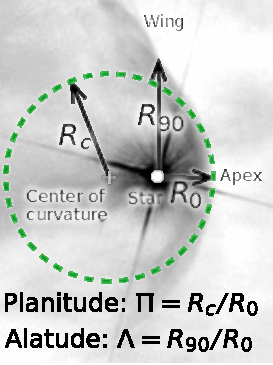
\includegraphics[width=0.6\linewidth]{figs/obs-shape-terminology}
  \caption[Terminology]{Terminology employed in this paper to describe
    bow shock shapes, following \citet[Paper~0]{Tarango-Yong:2018a}.}
  \label{fig:obs-shape-terminology}
\end{figure}

The shapes of stellar bow shocks are frequently compared with what has
become known as the \textit{wilkinoid} surface \citep{Cox:2012a},
which is the result of the idealized interaction between a spherical
wind and a plane-parallel stream in the hydrodynamic thin-shell
approximation.  Numerical approximations to this shape were used by
various authors \citep{Baranov:1971a, Mac-Low:1991a} before an elegant
analytic solution was found by \citet{Wilkin:1996a} and extended to
the case of interaction between two spherical winds
\citep{Canto:1996}.  In \citet[hereafter, Paper~0]{Tarango-Yong:2018a}
the study of bow shock shapes and their projection on the plane of the
sky was formalized. The term \textit{cantoid} was introduced for the
\citet{Canto:1996} family of shapes, together with \textit{ancantoid}
for a generalization to the case where one of the winds is
anisotropic, as is appropriate for the proplyds.  In addition, Paper~0
proposed the use of two dimensionless parameters, \textit{planitude}
and \textit{alatude}, to describe a general bow shock shape, which we
illustrate in Figure~\ref{fig:obs-shape-terminology}.  The planitude,
\(\Pi = R_c / R_0\), measures the flatness of the bow shock apex, where
\(R_0\) is the star--apex distance and \(R_c\) is the radius of
curvature measured at the apex.  The alatude,
\(\Lambda = R_{90}/R_0\), measures the openness of the bow shock wings,
where \(R_{90}\) is the lateral size of the bow, measured from the
star in the direction perpendicular to the star--apex direction.

In this paper, we investigate the shapes of stellar bow shocks by
calculating the distributions of planitude and alatude for different
classes of bow shock source.  The remainder of the paper is organized
as follows. In \S~\ref{sec:mid-infrared-arcs} we present an analysis
of the shapes of several hundred bow shock candidates associated with
OB stars from the \SI{24}{\um} survey of \citet{Kobulnicky:2016a}.
Our algorithm for automatically fitting and tracing the shapes is
described in \S~\ref{sec:autom-trac-fitt}, together with our ``star
rating'' system for evaluating the fit quality, while in
\S~\ref{sec:ob-shapes} we locate the sources on the planitude--alatude
plane.  In \S~\ref{sec:corr-size} we study the correlations amongst
non-shape parameters of the bow shock sources, such as angular size
and stellar magnitude, while in \S~\ref{sec:corr-shape} we explore the
correlations between these parameters and the planitude and alatude.  In
\S~\ref{sec:far-infrared-arcs} we compare with results for bow shocks
around cool luminous stars and in \S~\ref{sec:stat-emiss-line} we
compare with results for stationary emission-line arcs in the Orion
Nebula.  In \S~\ref{sec:discussion} we discuss the implications of our
findings for physical models of bow shock formation in the different
classes of sources, and in \S~\ref{sec:conclusion} we summarise our
results.  Further details of the statistical tests that we have
applied are provided in Appendix~\ref{sec:distr-p-values} and a simple
model for time-dependent oscillations of the bow shock surface is
presented in Appendix~\ref{sec:perturbed-bows}.

% Bowshocks from red supergiants \citep{Meyer:2014a}.  Simluations of AGB bows \citep{Villaver:2012a}, RSG \citep{Mohamed:2012a}


% Wolf Rayet stars give bigger bow shocks (e.g., WR~128 \citealp{Moffat:1998})

% Interaction of wind with photoevaporation flow \citep{Dyson:1975a}

% HMXRB in external galaxies, possible bowshock in LMC~X-1 \citep{Hyde:2017a}.

% Wolf-Rayet bow shock nebulae \citep{Dyson:1989a}

% Non-thermal radio emission from BD+43~3654 \citep{Benaglia:2010a}, has
% been searched for but

% Supersonic pulsar wind nebulae \citep{Kargaltsev:2017a}


%%% Local Variables:
%%% mode: latex
%%% TeX-master: "obs-bowshocks"
%%% End:

\clearpage
\section{Comparison with observations}
\label{sec:comp-with-observ}


Placing various classes of objects on the \(R_{90}\)--\(R_c\) plane:
\begin{itemize}
\item LL arcs
\item runaway O stars
\item AGB stars
\end{itemize}

\subsection{Mid-infrared arcs around early-type stars}
\label{sec:mid-infrared-arcs}

\begin{figure*}
  \setlength\tabcolsep{0pt}
  \begin{tabular}{ll}
    (a)
    & (b) \\
    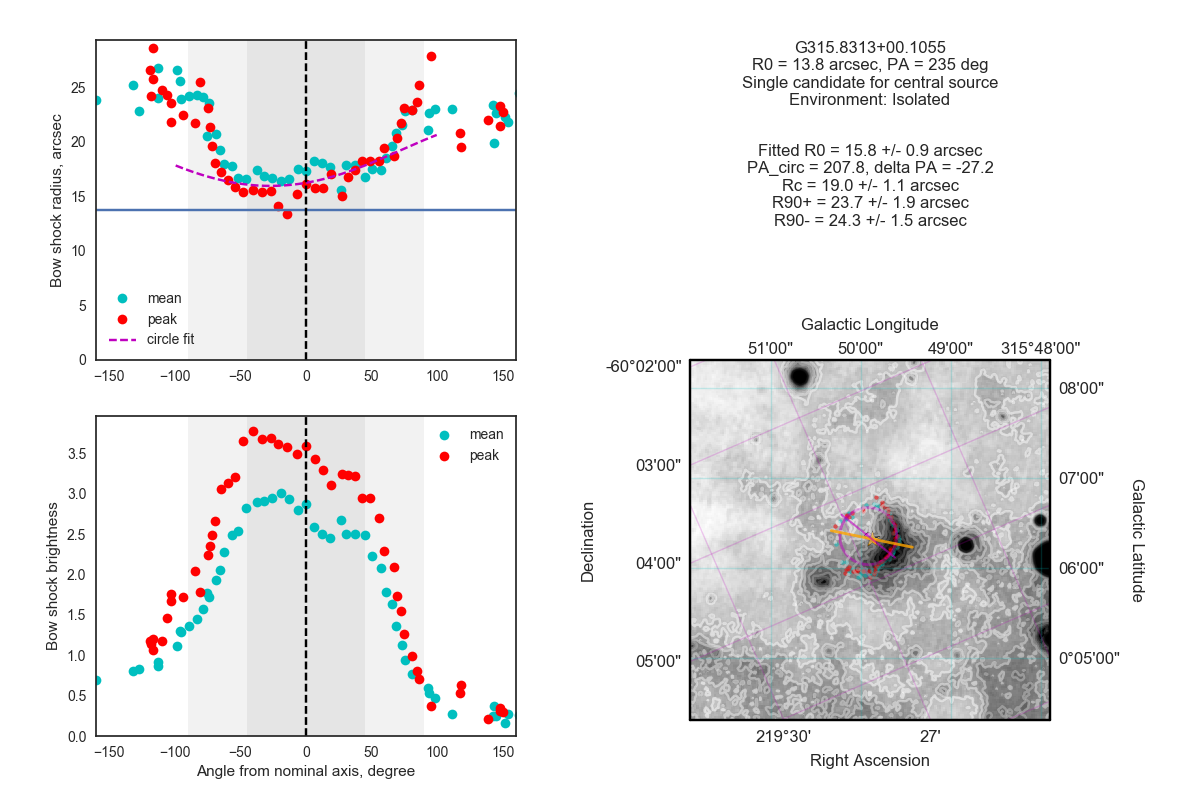
\includegraphics
    [width=0.5\linewidth, trim=20 15 30 10, clip]{figs/0510-3-star}
    & 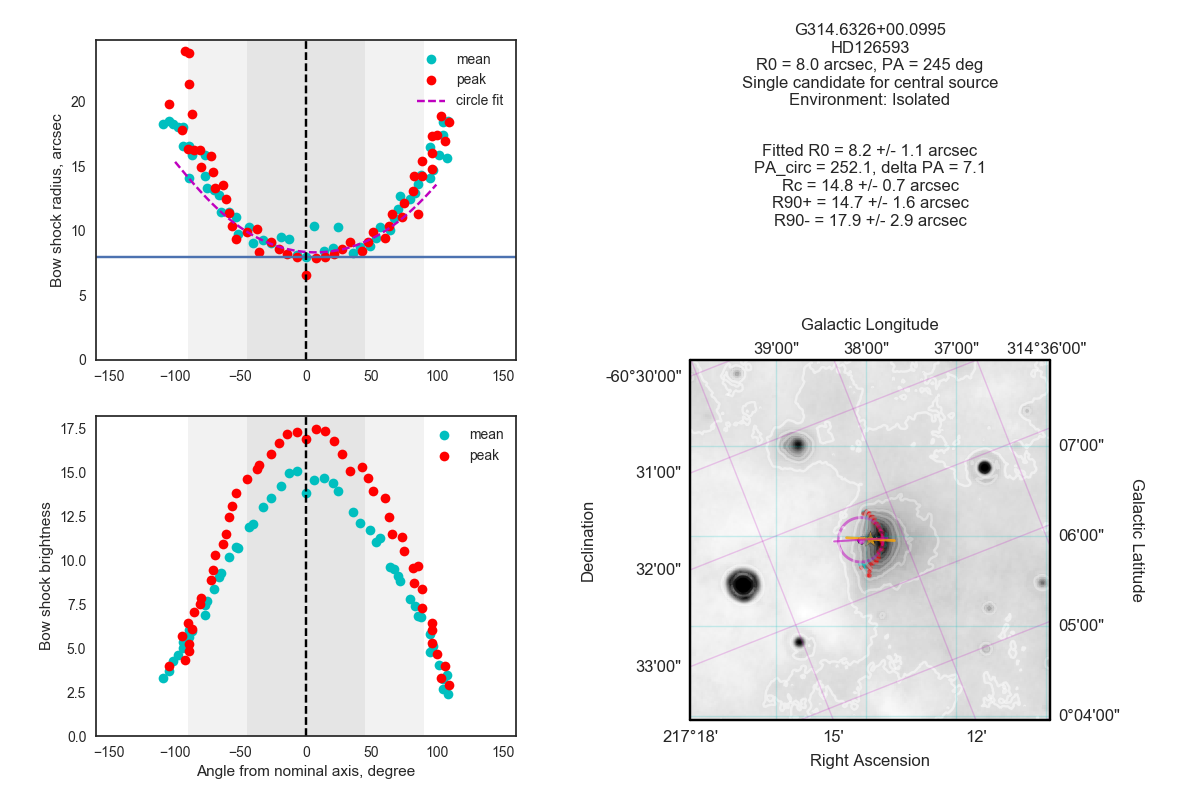
\includegraphics
      [width=0.5\linewidth, trim=20 15 30 10, clip]{figs/0506-4-star} \\
    (c)
    & (d) \\
    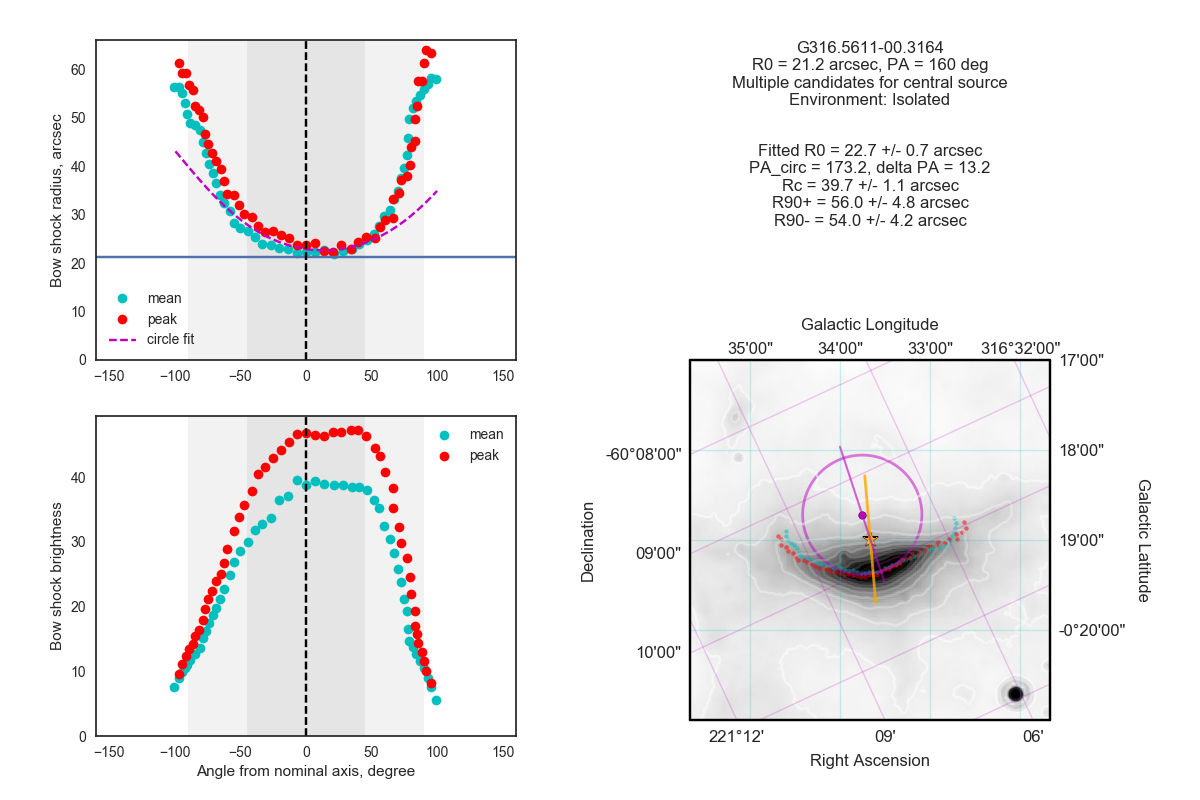
\includegraphics
    [width=0.5\linewidth, trim=20 15 30 10, clip]{figs/0517-5-star}
    & \multicolumn{1}{c}
      {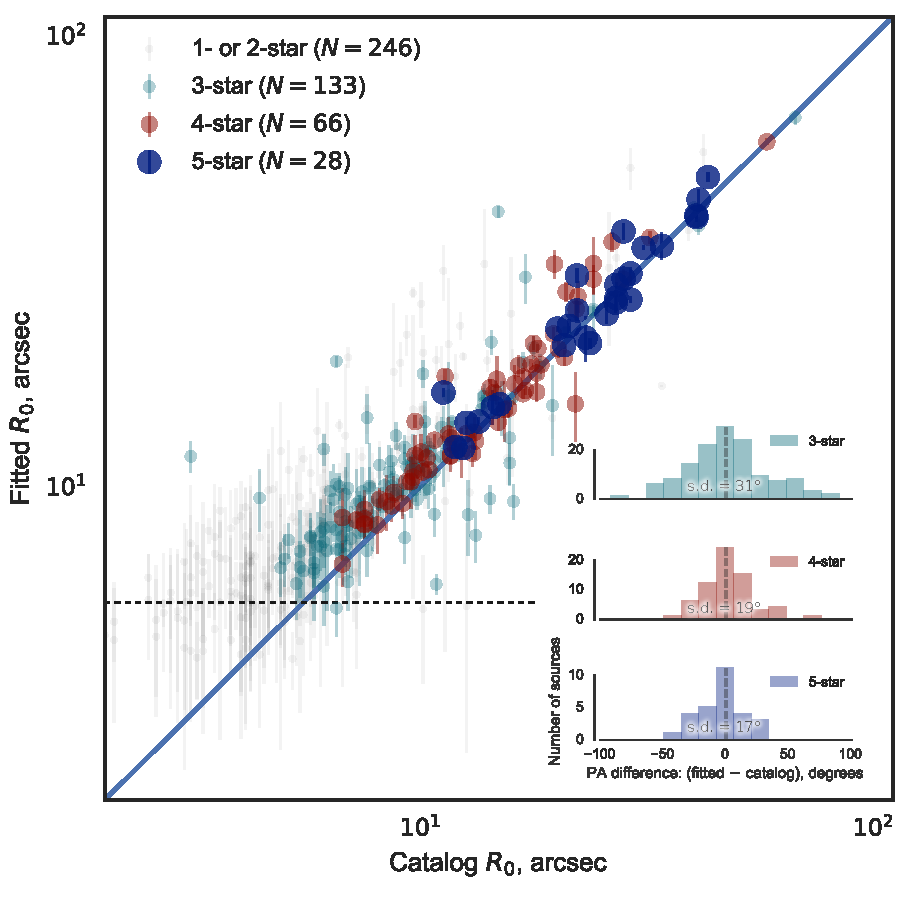
\includegraphics[width=0.35\linewidth, trim=20 20 20 20]
      {figs/mipsgal-r0-r0-plus-dPA-edited}}
  \end{tabular}
  \caption[]{Examples of typical fits to the bow shock shapes of
    MIPSGAL sources with different star ratings: (a) K510, 3-star
    rating; (b) K506, 4-star rating; (c) K517, 5-star rating.  Right
    panels of parts (a)--(c) show a 4\('\) square \SI{24}{\um} image,
    centered on each source.  Contours are ten linearly spaced levels
    between the median brightness of the entire image and the maximum
    brightness of the bow shock arc. Grids of galactic coordinates
    (light blue lines, parallel to the box sides) and equatorial
    coordinates (tilted magenta lines) are shown.  The stellar source
    and the bow shock axis, as determined by \citet{Kobulnicky:2016a}
    are indicated by an orange star and an orange line, respectively,
    where the line extends from \(-2 R_0\) to \(+2 R_0\).  The
    automatically traced arc shapes using the ``mean'' and ``peak''
    methods (see text) are shown by blue and red dots, respectively.
    The magenta circle shows the fit to the arc points within
    \(\pm 45^\circ\) of the nominal bowshock axis, with the magenta dot
    showing the center of curvature and the magenta line showing the
    fitted bow shock axis, which is the line passing through the
    source and the center of curvature.  Left panels of parts (a)--(c)
    show the radius measured from the source (upper panel) and
    brightness (lower panel) of the arc points, plotted as a function
    of angle \(\theta\) from the nominal bow shock axis, and with the same
    color coding as used on the image. Angular ranges of
    \(\theta = \pm 45\degr\) and \(\pm 90\degr\) are shown by gray shaded
    boxes In the upper panel, the \(R_0\) value tabulated by
    \citet{Kobulnicky:2016a} is shown by a horizontal blue line. (d)
    Comparison of the bow shock sizes (scatter plot) and position
    angles (inset histograms) determined from our fits with those
    tabulated by \citet{Kobulnicky:2016a} for the MIPSGAL sources.
    The horizontal dotted line on the main plot shows the MIPS
    \SI{24}{\um} point spread function FWHM of \(5.5\arcsec\).  The
    standard deviation (s.d.) of the position angle differences is
    shown on each inset histogram.}
  \label{fig:mipsgal-examples}
\end{figure*}


The most extensive observational sample of stellar bow shock nebulae
to date is a catalog of 709 arcs \citep{Kobulnicky:2016a} detected in
mid-infrared surveys of the Galactic Plane by the \textit{Spitzer
  Space Telescope} (\textit{SST}, \citealp{Werner:2004a}) and
\textit{Wide-field Infrared Survey Explorer} (\textit{WISE},
\citealp{Wright:2010a}).  These sources are believed to be powered by
the winds of early-type stars, which are either moving supersonically
through the interstellar medium (runaway stars,
\citealp{Gvaramadze:2008a}), or are interacting with a local bulk
flow, such as the champagne flow from a nearby \hii{} region (weather
vanes, \citealp{Povich:2008a}).


\subsubsection{Automatic tracing and fitting of bow shocks}
\label{sec:autom-trac-fitt}


In order to study the shapes of these bow shocks, we downloaded data
from the NASA/IPAC Infrared Science Archive archive\footnote{
  \url{http://irsa.ipac.caltech.edu/docs/program_interface/api_images.html}}
and extracted 4\arcmin{} square images in the \SI{24}{\um} bandpass of
the Multiband Imaging Photometer for \textit{Spitzer} (MIPS) centered
on each of the 471 \citet{Kobulnicky:2016a} sources that are covered
by the MIPSGAL \citep{Carey:2009a} survey, which includes most of the
sources with Galactic longitude within \(\pm 60\degr\) of the Galactic
center.

We developed a methodology for automatically tracing the arcs as follows:
\begin{enumerate}[1.]
\item Calculate arrays of celestial coordinates, \(C\), for each pixel
  of the image.
\item Using the central source coordinates, \(C_0\) and nominal
  bowshock radius, \(R_0\) from \citet{Kobulnicky:2016a}, construct a
  pixel mask that includes only those pixels with separations from the
  source that satisfy \(\frac12 R_0 \le |C - C_0| \le 3 R_0\).  This mask
  will be used for all subsequent operations, which serves to help
  avoid confusion from the star itself and other bright sources in the
  field of view.
\item Define a ``step-back'' point, \(C_1\), which is located at a
  separation \(2 R_0\) from the source, but in the opposite direction
  from the apex of the bow shock. That is, along a position angle
  180\degr{} from the nominal position angle, \(\text{PA}_0\), of the
  bow shock axis.  This point is at one end of the orange line shown
  superimposed on the bow shock images in
  Figure~\ref{fig:mipsgal-examples}.
\item Looping over a grid of 50 position angles, \(\text{PA}_k\),
  within \(\pm 60\degr\) of \(\text{PA}_0\), estimate the location of
  the arc along rays cast from the step-back point, using two
  different methods:
  \begin{enumerate}[(a)]
  \item The pixel with the peak brightness, with coordinates
    \(C_{k,\text{peak}}\) (red dots in
    Fig.~\ref{fig:mipsgal-examples}).
  \item The mean brightness-weighted separation from \(C_1\), with
    coordinates \(C_{k,\text{mean}}\) (light blue dots in
    Fig.~\ref{fig:mipsgal-examples}).
  \end{enumerate}
  For each \(\text{PA}_k\) in the grid, the calculation is performed
  over only those pixels that satisfy
  \(|\text{PA}(C, C_1) - \text{PA}_k| < \frac12 \delta\theta\), where
  \(\delta\theta = 120/50 = 2.4\degr\), which defines a thin radial wedge from
  \(C_1\).  The results are shown as red and blue dots superimposed
  on the images in Figure~\ref{fig:mipsgal-examples}. Each of the two
  methods, ``peak'' and ``mean'', works better in some objects and
  worse in others (according to the subjective judgment of
  ``correctly'' tracing the bow shock shape).  We therefore take the
  average by amalgamating all the \(C_{k,\text{peak}}\) and
  \(C_{k,\text{mean}}\) points into a single set, \(C_{k}\), for
  the following steps.
\item For each of the points \(C_{k}\), determine the radial
  separation from the central source, \(R_k = |C_k - C_0|\) and the
  angle from the bow shock axis about the central source
  \(\theta_k = \text{PA}(C_k, C_0) - \text{PA}_0\).  These are plotted in
  the upper left panels of Figure~\ref{fig:mipsgal-examples}.  Note
  that, even though the rays are cast from the step-back point \(C_1\)
  within \(\pm 60\degr\) of \(\text{PA}_0\), the angles \(\theta_k\) are
  measured from the source, \(C_0\), which is closer to the bow shock
  than \(C_1\) and therefore \(|\theta_k|\) can be much larger than
  \(60\degr\).
\item Make our own estimate of the axial size, \(R_0\), of the bow
  shock by calculating the mean of \(R_k\) over all points \(C_k\)
  with \(|\theta_k| \le 10\degr\).  Note that this is distinct from the
  nominal value of \(R_0\) given in the \citet{Kobulnicky:2016a}
  catalog, which was ``measured by eye''.  We denote by
  \(\epsilon(R_0)\) the standard deviation of the \(R_k\) that go into
  calculating \(R_0\).\label{step:R0}
\item Estimate the radius of curvature, \(R_c\), by fitting a circle
  to all those points within \(\pm 45\degr\) of the nominal axis
  (\(|\theta_k| < 45\degr\)), but after excluding any point with
  \(R_k < \frac12 R_m\) or \(R_k > 2 R_m\), where \(R_m\) is the median
  \(R_k\) for \(|\theta_k| < 45\degr\).
\item Determine two separate estimates, \(R_{90+}\) and \(R_{90-}\),
  of the perpendicular radius, \(R_{90}\), by taking the mean of
  \(R_k\) over all points \(C_k\) with
  \(|\theta_k - 90\degr| \le 10\degr\) for \(R_{90+}\), and with
  \(|\theta_k + 90\degr| \le 10\degr\) for \(R_{90-}\).  The average of the
  two standard deviations of the \(R_k\) that contribute to
  \(R_{90+}\) and \(R_{90-}\) is denoted by \(\epsilon(R_{90})\).\label{step:R90}
\end{enumerate}


\subsubsection{Subjective evaluation of the fit quality}
\label{sec:subj-eval-fit}


After these automatic steps, we subjectively evaluate the results by giving a star rating to each source:

\paragraph*{0 stars} The fitting algorithm failed for some reason. 

\paragraph*{1 star} The fit was formally successful, but the results
for \(R_c\) or \(R_{90}\) are far removed from what a human would
predict by looking at the image.  For example, in the smallest
bowshocks, which are only marginally resolved by Spitzer's 6\arcsec{}
beam, the dispersion in \(R_k\) can be a significant fraction of
\(R_0\), in which case our algorithm tends to erroneously favor
\(R_c < R_0\).

\paragraph*{2 stars} The fit results are not totally outlandish, but
nonetheless some problem is apparent that casts doubt on their
reliability.  For example, a double-shell structure to the bow shock
that leads to large differences between the ``peak'' and ``mean''
methods, or point sources near to the bow shock that interfere with
the tracing procedure.
  
\paragraph*{3 stars} A good fit, but where the dispersion in \(R_k\)
and/or the asymmetry in the bow shock reduces the precision in the
determination of \(R_c\) and \(R_{90}\), giving subjectively estimated
uncertainties around the 20\% level.  An example of a 3-star fit is
shown in Figure~\ref{fig:mipsgal-examples}a.

\paragraph*{4 stars} A high quality fit, with subjectively estimated
uncertainties in \(R_c\) and \(R_{90}\) around the 10\% level. An
example of a 4-star fit is shown in
Figure~\ref{fig:mipsgal-examples}b.

\paragraph*{5 stars} The highest-quality fit, usually corresponding to
large, sharply defined bow shocks, whose shape is determined with high
precision. An example of a 5-star fit is shown in
Figure~\ref{fig:mipsgal-examples}c.

\bigskip
%
Figure~\ref{fig:mipsgal-examples}d compares the bow shock size,
\(R_0\), determined by our fits (vertical axis) with the corresponding
value given in the \citet{Kobulnicky:2016a} catalog (horizontal axis).
For most sources with 3-star or higher rating, the two estimates agree
to within \(\pm 20\%\), but there are a small number of sources with a
discrepancy of more than a factor of two.  In all cases that we
checked, we believe that our estimates of \(R_0\) are more accurate
than those in the catalog.  It is apparent that the star ratings are
correlated with the bow shock size, with larger bow shocks tending to
receive higher ratings, although there is considerable overlap.  In
particular, most of the 1- and 2-star sources are close to the
resolution limit of the MIPSGAL \SI{24}{\um} images (\(6\arcsec\),
indicated by the dotted horizontal line in te figure).

\begin{figure*}
  \centering
  \begin{tabular}{ll}
    (a) & (b) \\
    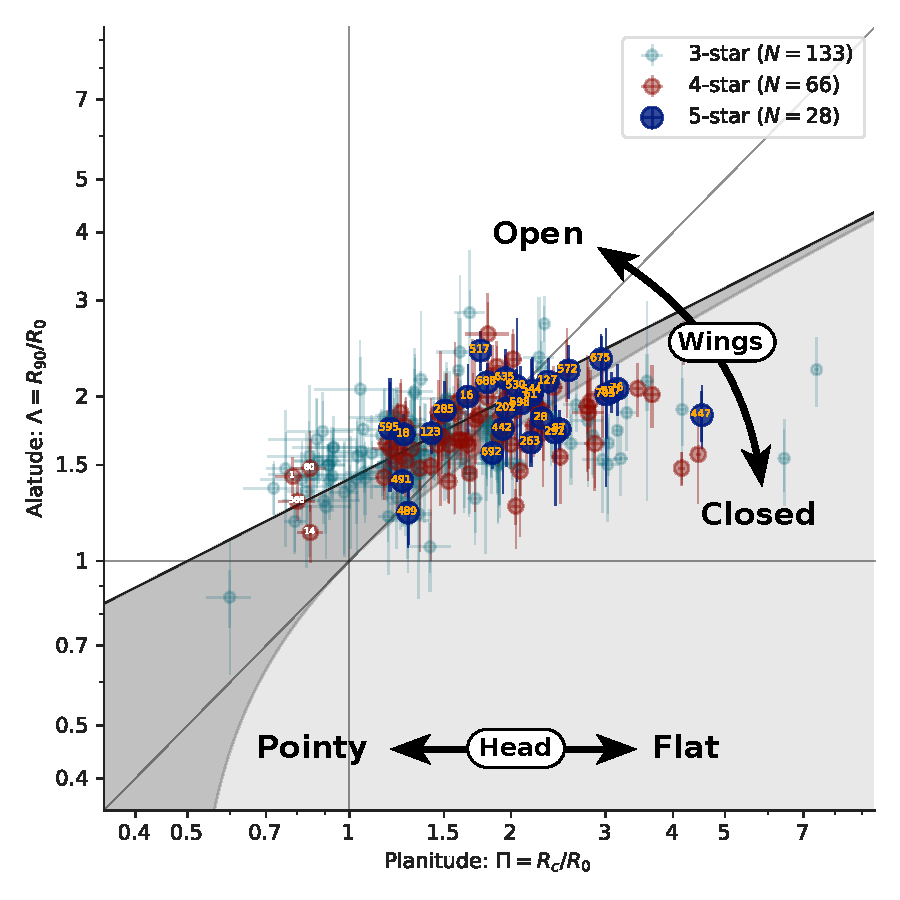
\includegraphics[width=0.45\textwidth, trim=0 0 30 0]
    {figs/mipsgal-Rc-R90-zoom-annotated}
        & 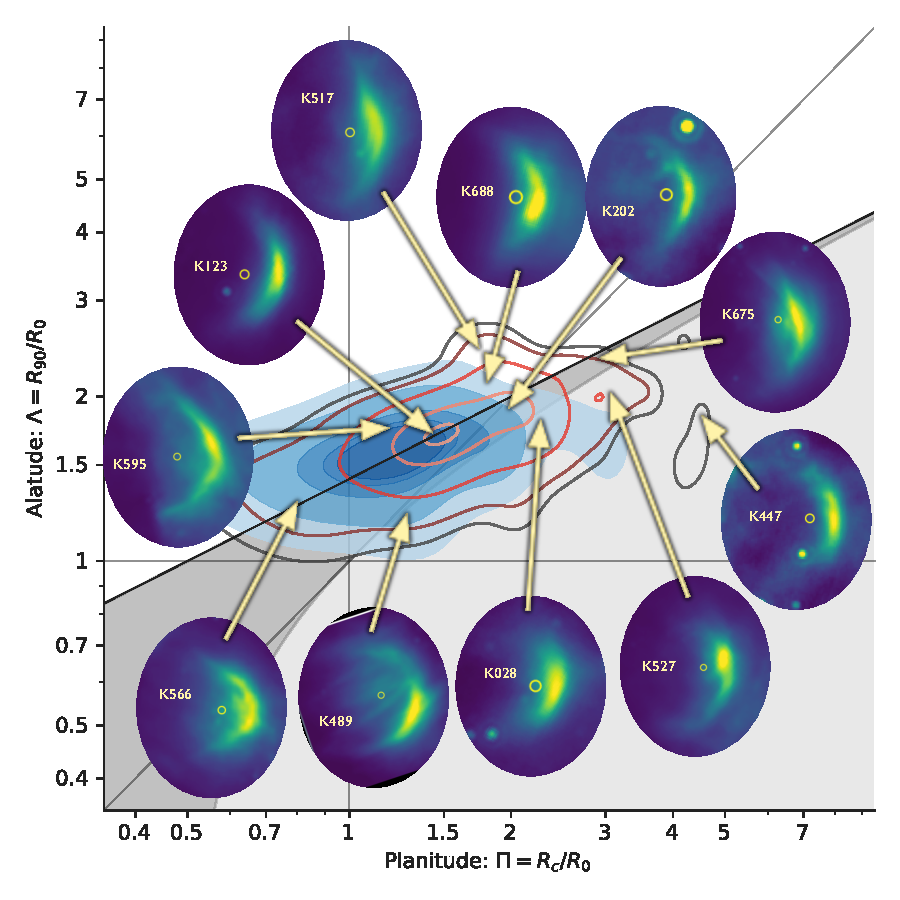
\includegraphics[width=0.45\textwidth, trim=0 0 30 0]
          {figs/mipsgal-Rc-R90-thumbnails} 
  \end{tabular}
  \caption[]{MIPSGAL sources on the bow shock shape diagnostic diagram
    of dimensionless radius of curvature versus perpendicular radius.
    The regions corresponding to different classes of cuadrics are
    shown by shading (see \S~\ref{sec:conic}): oblate spheroids (light
    gray background); prolate spheroids (darker gray background);
    paraboloids (curved black line); hyperboloids (white background).
    (a) Individual sources with bow shock fit quality rating of 3-star
    or above.  All 5-star sources plus those 4-star sources with
    \(R_c/R_0 < 1\) are labelled with their \cite{Kobulnicky:2016a}
    catalog number.  Horizontal error bars do not directly reflect the
    uncertainty in \(R_c/R_0\) but are instead simply the standard
    deviation from the circle fit of bowshock points \(R_k\) within
    \(\pm 45\degr\) of the axis.  Values on the vertical axis
    represent the average of \(R_{90+}\) and \(R_{90-}\), with thin
    vertical error bars showing the difference between \(R_{90+}\) and
    \(R_{90-}\), and thick vertical error bars showing the rms
    dispersion of \(R_k\) about these values for bow shock points
    within \(\pm 10\degr\) of the \(+90\degr\) and \(-90\degr\)
    directions.  (b) Kernel density estimator (KDE) of the
    distribution for 3-star sources (blue, filled contours) and 4-
    plus 5-star sources (orange/brown, unfilled contours).  The KDE
    uses an anisotropic gaussian kernel with bandwidths of
    \(0.18 \times 0.12\). Thumbnail images of representative 4- and 5-star
    sources at different points on the \(R_c\)--\(R_{90}\) plane are
    also shown. The angular scale of each image is indicated by a
    yellow circle of diameter \(7.5''\), centered on the stellar
    source.}
  \label{fig:mipsgal-shapes}
\end{figure*}

In the following analysis, only those sources with a 3-star or higher
rating are used.  These comprise approximately half (227 out of 471)
of all the MIPSGAL arc sources.  In some cases of poor and failed
fits, there is nothing apparently ``wrong'' with the source itself,
and it is likely that minor tweaks to the methodology would improve
matters, but we have elected not to do so, in order to maintain a
uniform methodology across all sources.

The inset of Figure~\ref{fig:mipsgal-examples}d shows histograms of
the difference between the position angle, \(\text{PA}_0\) determined
by our fits and that listed in \citet{Kobulnicky:2016a}.  Although
observational uncertainties undoubtedly contribute in part, the
differences are mainly due to real asymmetries in the bow shocks,
especially for the 4- and 5-star sources.  The
\citeauthor{Kobulnicky:2016a} catalog \(\text{PA}_0\) values are
mostly sensitive to the orientation of the bow shock wings, whereas
our fitted \(\text{PA}_0\) values are determined by the point in the
bow shock head that is closest to the stellar source.  For this
reason, we use the catalog \(\text{PA}_0\) values for defining the
axis when measuring \(R_{90+}\) and \(R_{90-}\). On the other hand,
the fitted values of \(\text{PA}_0\) are better correlated with the
position of the bow shock's brightness peak, as is apparent in the
lower left panels of Figure~\ref{fig:mipsgal-examples}a and c.

\subsubsection{OB bow shock shapes on the diagnostic plane}
\label{sec:ob-shapes}

The derived bowshock shapes of all the 3-, 4-, and 5-star sources are
shown in Figure~\ref{fig:mipsgal-shapes} on the plane of \(R_c/R_0\)
versus \(R_{90} / R_0\).  Panel a shows the individual points
superimposed on the theoretical results for quadrics of revolution
(see figure caption and \S~\ref{sec:conic}), while panel b shows
contours of the kernel density estimator (KDE, see
\citealp{Leiva-Murillo:2012a, Scott:2015a}) of the two-dimensional
distribution of points on the \(R_c\)--\(R_{90}\) plane.  The
horizontal axis corresponds to the shape of the head of the bow shock
near its apex, ranging from sharper, pointier shapes with
\(R_c/R_0 < 1\) to flatter, snubber shapes with \(R_c/R_0 \gg 1\), where
it must be understood that all judgments of sharpness/flatness are
with respect to the axial separation, \(R_0\), between the source and
the bow shock apex.  The vertical axis corresponds to the shape of the
bow shock wings, ranging from closed ``C'' shapes for smaller values
of \(R_{90} / R_0\) to open ``V'' shapes for larger values of
\(R_{90} / R_0\).  The boundary between closed and open corresponds to
the paraboloids, and is shown by the solid curved line that divides
the shaded from the unshaded regions of the graph.

The KDE contours in Figure~\ref{fig:mipsgal-shapes}b show that the
distribution of 3-star sources is very similar to that of 4- and
5-star sources, although the higher-rated sources are shifted slightly
to the upper right.  Possible reasons for this are discussed in
\S~\ref{sec:corr-shape} below.
% This is probably due to higher-rated sources
% being on average bigger, as will be discussed further below.
The bulk of the sources are concentrated around the paraboloid line,
with \(1 < R_c/R_0 < 2.5\), and \(1.2 < R_{90}/R_0 < 2\).  But
significant minorities are found in three other regions: (1)~a clump
with \(R_c/R_0 \la 1\); (2)~a vertical spur towards higher \(R_{90}\)
at \(R_c/R_0 \approx 2\); and (3)~a broad horizontal tail towards higher
\(R_c\) at \(R_{90}/R_0 \la 2\).


\subsubsection{Correlation between bow shock size and other parameters}
\label{sec:corr-size}

\begin{figure*}
  \centering
  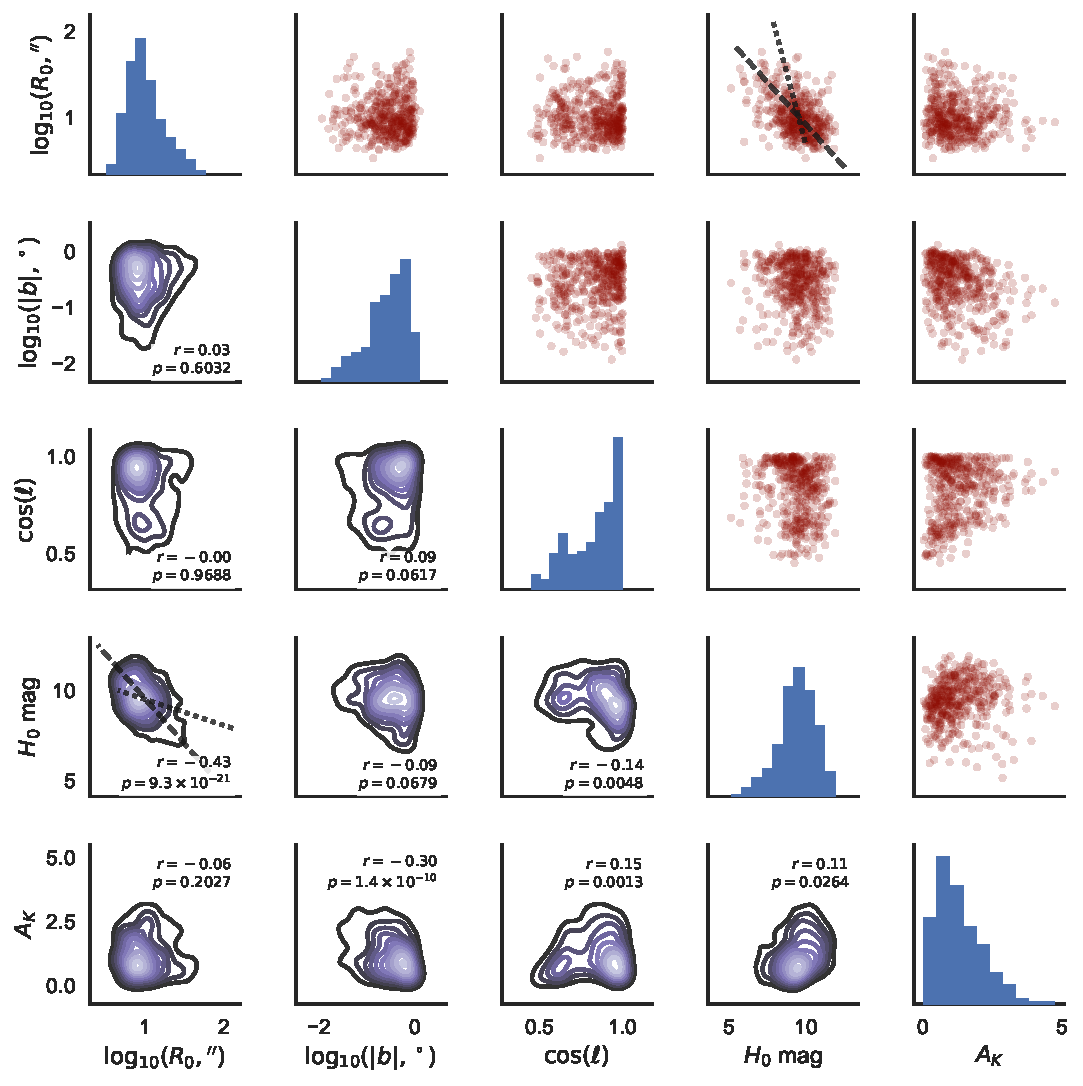
\includegraphics[width=0.8\textwidth]{figs/mipsgal-pairplot}
  \caption[]{Matrix of pair plots that illustrate distributions of and
    correlations between the non-shape parameters of all MIPSGAL bow
    shock sources from \citet{Kobulnicky:2016a}.  Plots on the leading
    diagonal show histograms of the following parameters: bow shock
    angular size, \(\log_{10} R_0\); Galactic latitude,
    \(\log_{10}|b|\); Galactic longitude, \(\cos \ell\);
    extinction-corrected \(H\)-band magnitude of the stellar source,
    \(H_0\); \(K\)-band extinction, \(A_K\).  Scatter plots in the
    upper triangle show the joint distribution of each pair of
    parameters.  These are repeated in the lower triangle but showing
    the KDEs of the joint distributions, which are annotated with the
    Pearson linear correlation coefficient, \(r\), for each pair. The
    straight lines shown superimposed on the plots of stellar magnitude
    versus bowshock size correspond to toy model results for the same star
    at a sequence of distances (dashed lines) and a sequence of
    stellar luminosities at a fixed distance (dotted lines).  See text
    for details. }
  \label{fig:mipsgal-pairplot}
\end{figure*}

In Figure~\ref{fig:mipsgal-pairplot} we show the distributions over
all MIPSGAL bow shock sources of the bow shock size, Galactic
coordinates, extinction-corrected stellar source magnitude, and dust
extinction.  For the bow shock size, \(R_0\), we use the results from
our model fitting rather than the values given in the
\citet{Kobulnicky:2016a} catalog, but the distribution is very
similar, as can be seen by comparing the top-left plot of
Figure~\ref{fig:mipsgal-pairplot} with \citeauthor{Kobulnicky:2016a}'s
Figure~8.

The catalog gives the \(K\)-band extinction, \(A_K\), derived using
the method of \citet{Majewski:2011a}, but that assumes an intrinsic
color of \((H - [\SI{4.5}{\um}])_0 = +0.08\) magnitudes, which is too
red if the sources are assumed to be OB stars.  We therefore re-derive
\(A_K\) from the catalog magnitudes combined with the
\citet{Indebetouw:2005a} reddening law, but assuming
\((H - [\SI{4.5}{\um}])_0 = -0.1\) magnitudes, which is more typical
of early type stars.  This does not make very much difference (compare
the top-right plot of our Fig.~\ref{fig:mipsgal-pairplot} with
\citeauthor{Kobulnicky:2016a}'s Fig.~9), but it does eliminate some of
the apparent negative extinctions that are found in the catalog.  The
same reddening law gives \(A_H = 1.55 A_K\), and this is used to
derive extinction-corrected \(H\)-band apparent magnitudes, \(H_0\).

\begin{figure*}
  \centering
  \begin{tabular}{ll}
    (a) & (b) \\
    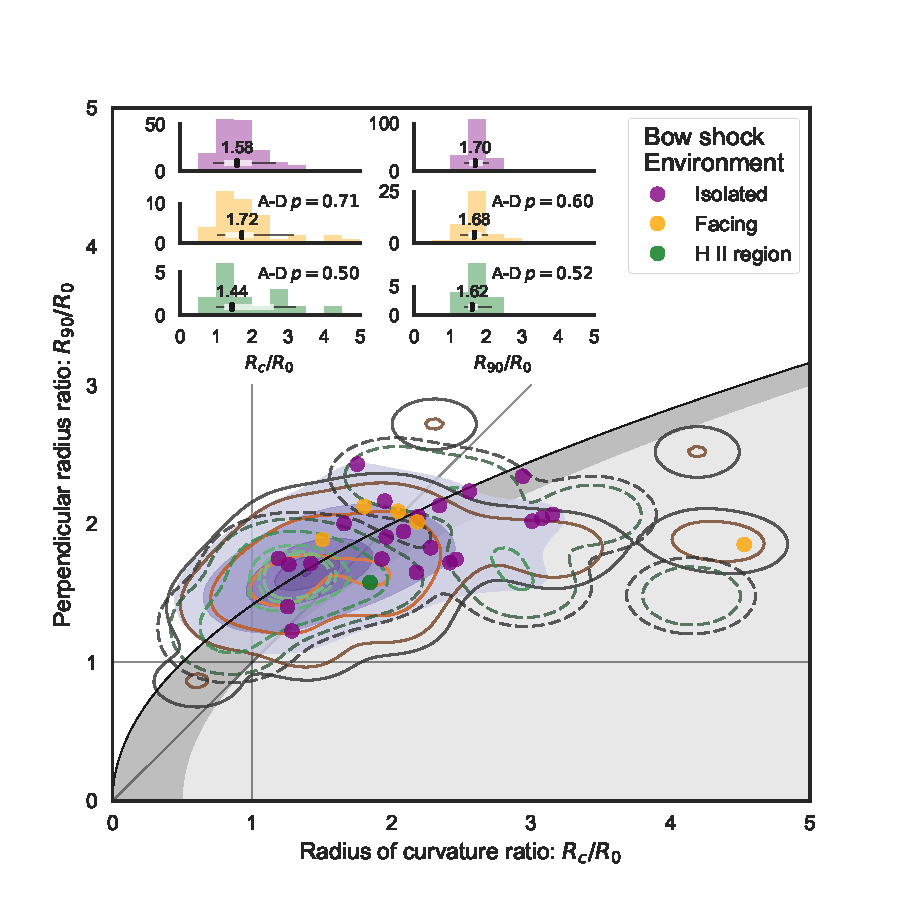
\includegraphics[width=0.45\textwidth]{figs/mipsgal-Rc-R90-environment} &
    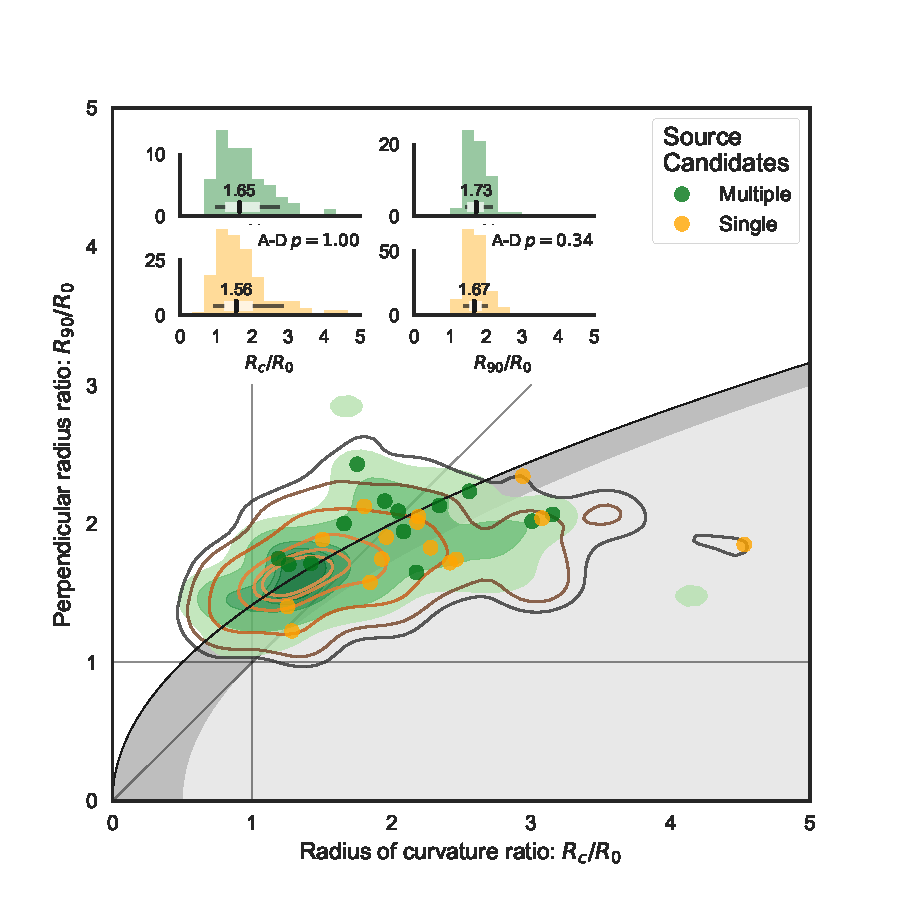
\includegraphics[width=0.45\textwidth]{figs/mipsgal-Rc-R90-candidates} 
  \end{tabular}
  \caption[]{Example comparisons between the distribution of bowshock
    shapes when the sources are divided into two or more sub-samples
    according to the value of a categorical parameter.  Contours show
    the KDE of the distribution of each sub-sample for all 3-, 4-, and
    5-star sources, while filled circle symbols show 5-star sources
    only. Inset histograms show the marginal distributions on the two
    shape axes. (a)~Source environment, divided into three
    sub-samples: ``Isolated'' (purple symbols and purple filled
    contours), ``Facing \hii{} region or \SI{8}{\um} bright-rimmed
    cloud'' (orange symbols and orange-brown hollow continuous
    contours), and ``Within \hii{} region'' (green symbols and green
    hollow dashed contours). (b)~Uncertainty in stellar source
    identification, divided into two sub-samples: ``Multiple
    candidates for stellar source'' (green symbols and green filled
    contours) and ``Single candidate for stellar source'' (orange
    symbols and orange-brown hollow continuous contours).}
  \label{fig:mipsgal-uncorrelated}
\end{figure*}

The most significant linear correlation between any pair of parameters
in Figure~\ref{fig:mipsgal-pairplot} is that between bow shock size
and stellar source brightness: \(H_0\) versus \(\log_{10} R_0\), with
correlation coefficient \(r = -0.43\).  The distribution of \(H_0\)
depends on the absolute magnitude, \(M_H\), and the distance, \(d\),
to the source.  It is likely that variation in \(d\) is the more
important of the two because \(M_H\) changes relatively little for
main-sequence OB stars, ranging from \(M_H \approx -4\) (early-O) to
\(M_H \approx -1.5\) (mid-B).  This is because part of the increase in
bolometric luminosity, \(L\), as one ascends the main sequence is
offset by an increase in the effective temperature,
\(T_{\text{eff}}\), which shifts the peak of the stellar spectrum
farther away from the \(H\)~band, resulting in
\(L_H \propto L / T_{\text{eff}}^3 \sim L^{0.53}\), where the last step uses
the upper main-sequence mass--luminosity and mass--radius scalings from
\citet{Eker:2015a}. It is true that evolved OB supergiants can be much
brighter, reaching \(M_H \approx -7\), but such stars are expected to be
rare.  Assuming a B2V star (\(M_H = -2\)), then the observed range
\(H_0 = 5\)--\(12\) corresponds to distances
\(d = 100\)--\SI{6300}{pc}, and the histogram peak at
\(H_0 \approx 9.5\) corresponds to \(d \approx \SI{2000}{pc}\), which is all
perfectly reasonable.

Turning now to the distribution of bow shock angular size, \(R_0\),
this will also be affected by distance to at least some degree, since
for a constant physical size the angular size will vary as
\(R_0 \propto d^{-1}\).  For instance, if we assume that the physical size
of all bow shocks is \SI{0.1}{pc} and the absolute magnitude of all
stars is \(M_H = -2\), as above, then we find the relation
\(H_0 = 14.57 - 5 \log_{10} R_0\) if \(R_0\) is measured in
arcseconds. This is shown as a dashed line on the relevant panels of
Figure~\ref{fig:mipsgal-pairplot} for values of \(R_0\) that
correspond to \(d = \SI{300}{pc}\) to \SI{8000}{pc}.  It can be seen
that this relation is in excellent agreement with the linear trend in
the data. On the other hand, the correlation coefficient of
\(r = -0.43\) means in broad terms that only a fraction
\(r^2 \approx 20\%\) of the total variance in \(H_0\) is ``explained'' by
changes in \(R_0\), and vice~versa, implying that one or both of
\(H_0\) and \(R_0\) is only a very imperfect proxy for \(d\).  We have
already seen that the spread in \(H_0\) probably \emph{is} mostly due
to a spread in distance, rather than a spread in \(H\)-band stellar
luminosity.  If this is true, it follows that it is \(R_0\) that
depends only weakly on \(d\) and is more influenced by other factors.

One such factor is the stellar/environmental momentum-loss ratio,
\(\beta\), between the two supersonic flows that form the bow shock.  All
other things being equal, we have \(R_0 \propto \beta^{1/2}\) for
\(\beta \ll 1\), as is typically the case.  If the environment flow is
constant and the OB star wind has mass-loss rate \(\dot{M}\) and
terminal velocity \(V_\infty\), then
\(\beta \propto \dot{M}{V_\infty}\).  Empirical and theoretical studies of hot star
winds (e.g., \citealp{Puls:1996a}) imply
\(\dot{M}{V_\infty} \sim L^{1.88} R^{-1/2} \sim L^{1.80} \sim L_H^{3.40}\), where
the final two steps apply only to main-sequence stars and again use
the relations of \citet{Eker:2015a}.  If we assume as above that a B2V
star with \(M_H = -2\) has a bow shock physical size of \SI{0.1}{pc},
and consider a sequence of stars with varying \(H\)-band luminosities
but all at a fixed distance of \(d = \SI{2000}{pc}\), then we find the
relation \(H_0 = 8.02 - 1.49 \log_{10} R_0\).  This is shown as a
dotted line in the relevant panels of
Figure~\ref{fig:mipsgal-pairplot} for the absolute magnitude range
\(M_H = -3.6\) (O6V) to \(M_H = -1.5\) (B5V).  It can be seen that
this relation does not match the linear trend in the data, and
predicts a much larger spread in \(R_0\) over a narrow range in
\(H_0\) than is observed.  This could mean one of two things: first,
it may be that the range of stellar luminosities is significantly
narrower than we have supposed, implying that B stars vastly outnumber
O stars among the sources.  Alternatively, there may be a positive
correlation between the stellar luminosity and the momentum of the
environmental flow, with the result that \(\beta\) varies less steeply
with \(L_H\) than we have assumed.  That could arise if more luminous
stars were preferentially found in denser environments, or, in the
case of runaways, if more luminous stars tended to be faster moving.

A third factor that may influence \(R_0\) is the inclination, \(i\),
of the bow shock axis with respect to the plane of the sky.
Figure~\ref{fig:quadric-projection}b shows that for \(R_c > 1\), then
the projected \(R_0'\) becomes larger than the true \(R_0\) as \(|i|\)
increases.  This is further illustrated in
Figure~\ref{fig:projected-R90-Rc-snapshots} for simple quadric shapes
(spheroids, paraboloids, hyperboloids) and in
Figure~\ref{fig:thin-shell-R90-Rc-snapshots} for the carawilkinoids
and ancarawilkinoids.  It can be seen that the effect is relatively
modest for bow shocks with projected shapes falling in the range
\(1 < R_c/R_0 < 3\) and \(R_{90}/R_0 < 3\), as the vast majority of
our observed sources do.  The increase in \(R_0\) is no more than a
factor of 2 to 3 for moderate inclinations of \(30\) to \(60\degr\),
although it can reach a factor of 5 to 10 for some shapes at more
extreme inclinations.

%% Maybe talk about the other correlations later if we have time

\subsubsection{Correlation between bow shock shape and other parameters}
\label{sec:corr-shape}
\begin{figure*}
  \centering
  \begin{tabular}{ll}
    (a) & (b) \\
    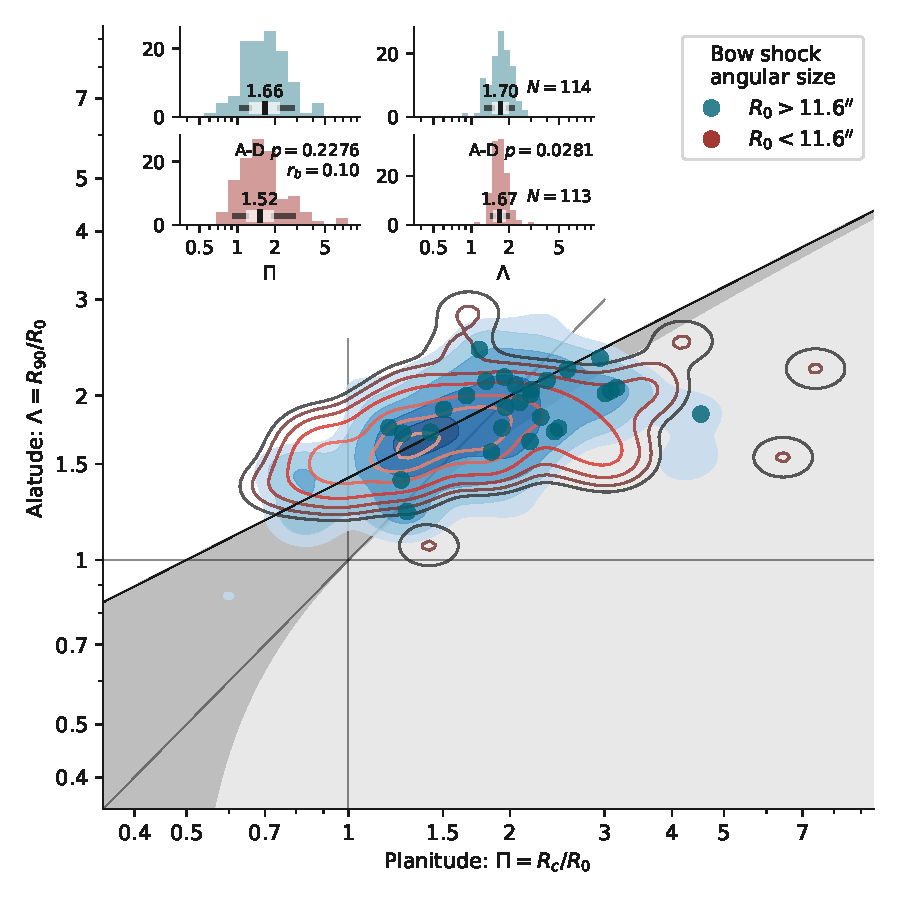
\includegraphics[width=0.45\textwidth]{figs/mipsgal-Rc-R90-R0} &
    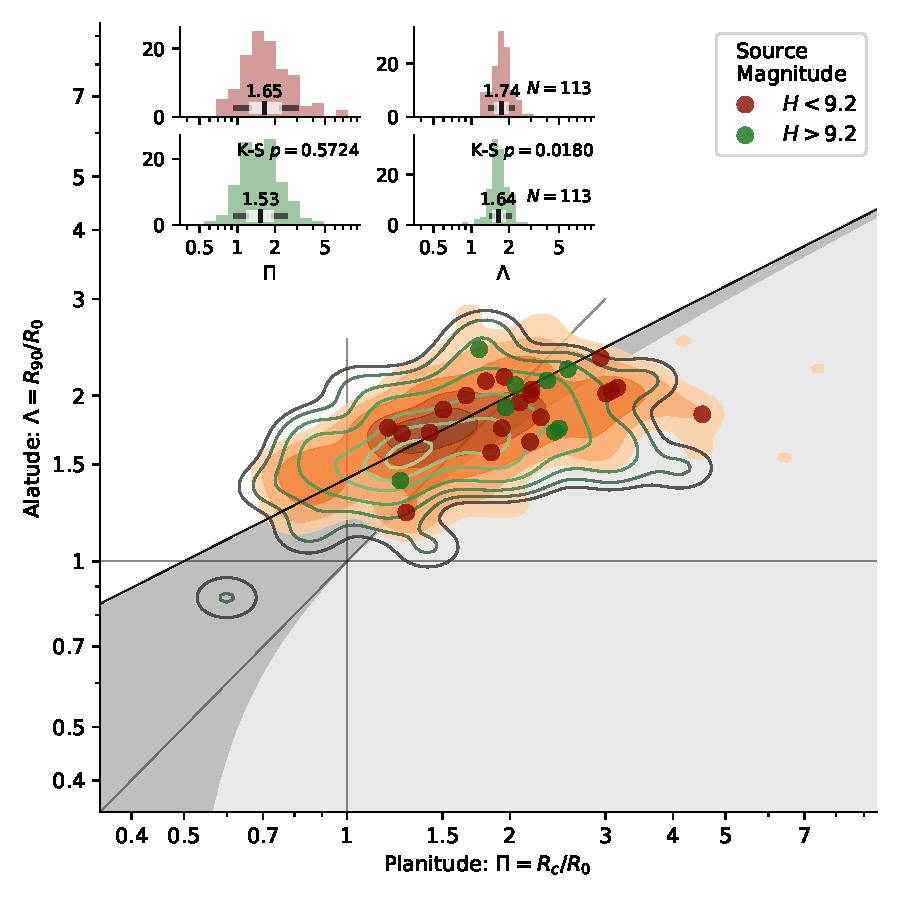
\includegraphics[width=0.45\textwidth]{figs/mipsgal-Rc-R90-Mag} 
  \end{tabular}
  \caption[]{As Fig.~\ref{fig:mipsgal-uncorrelated} but for median
    splits of continuous parameters. (a)~Bow shock angular size,
    \(R_0\), divided into two equal-sized sub-samples: large (blue
    symbols and blue filled contours) and small (red symbols and red
    hollow contours).  (b)~Extinction-corrected \(H\)-band magnitude
    of the stellar source, divided into two equal-sized sub-samples:
    bright (red symbols and orange filled contours) and faint (green
    symbols and green hollow contours).}
  \label{fig:mipsgal-correlated}
\end{figure*}

\begin{figure}
  \centering
  \setlength\tabcolsep{0pt}
  \begin{tabular}{ll}
    (a) & (b) \\
    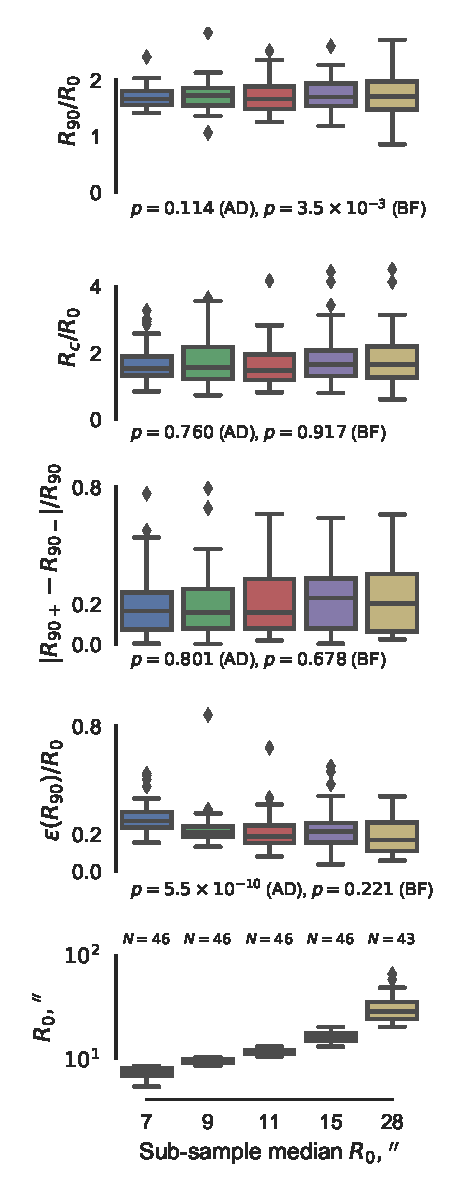
\includegraphics[height=1.167\linewidth]
    {figs/mipsgal-boxplot-Rc-R90-versus-R0}
        & 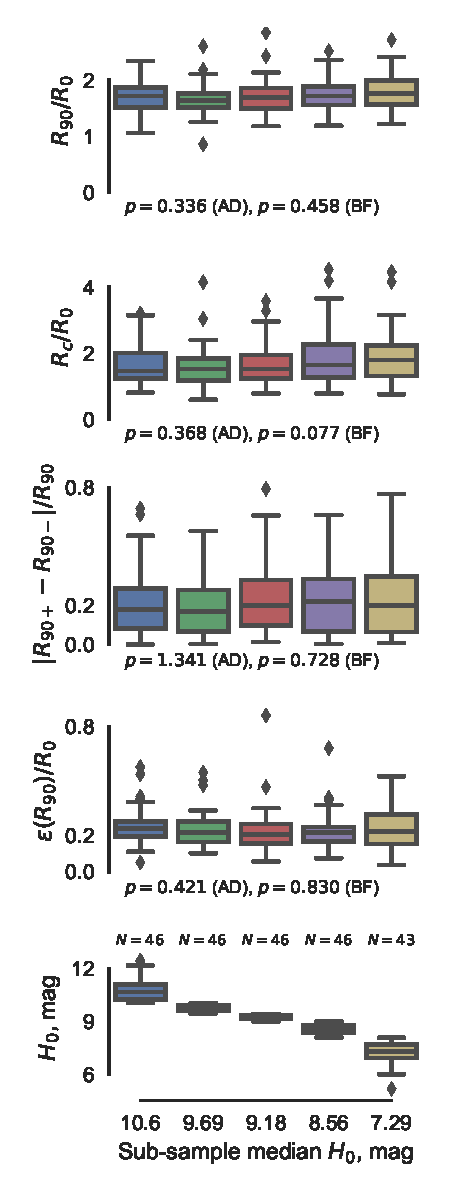
\includegraphics[height=1.167\linewidth]
          {figs/mipsgal-boxplot-Rc-R90-versus-H0}
  \end{tabular}
  \caption{(a) Box plots of the distributions of bow shock shape
    parameters, \(R_c/R_0\) and \(R_{90} / R_0\), together with a
    measure of the tail asymmetry, \(|R_{90+} - R_{90-}| / R_{90}\),
    after partitioning on the bow shock size, \(R_0\).  All 3-, 4-,
    and 5-star sources are sorted according to \(R_0\) and divided
    into 5 non-overlapping sub-samples of roughly equal size, each
    labelled by their median value of \(R_0\) in arcseconds, as
    illustrated in the lower panel.  The colored boxes show the
    interquartile range, with the median indicated by a horizontal
    line, the 1st-to-9th interdecile range by error bars, and outliers
    by diamonds.  A 5-sample Anderson--Darling test and Brown--Forsythe
    test is performed for each dependent variable, with resultant
    \(p\)-value given at the bottom of each panel.   It is apparent
    that the dispersion in \(R_{90} / R_0\) (upper panel) increases
    systematically with \(R_0\), although the central value is roughly
    constant.  No clear systematic changes are apparent in
    \(R_c / R_{90}\) (middle panel).  (b)~As (a), but partitioning on
    the extinction-corrected \(H\)-band magnitude, \(H_0\).  Note that
    sub-samples are plotted in order of \textit{decreasing} magnitude
    to allow comparison between (a) and (b), given the negative
    correlation between \(H_0\) and \(R_0\) (see
    Fig.~\ref{fig:mipsgal-pairplot}).}
  \label{fig:mipsgal-boxplot}
\end{figure}

\begin{figure}
  \centering
  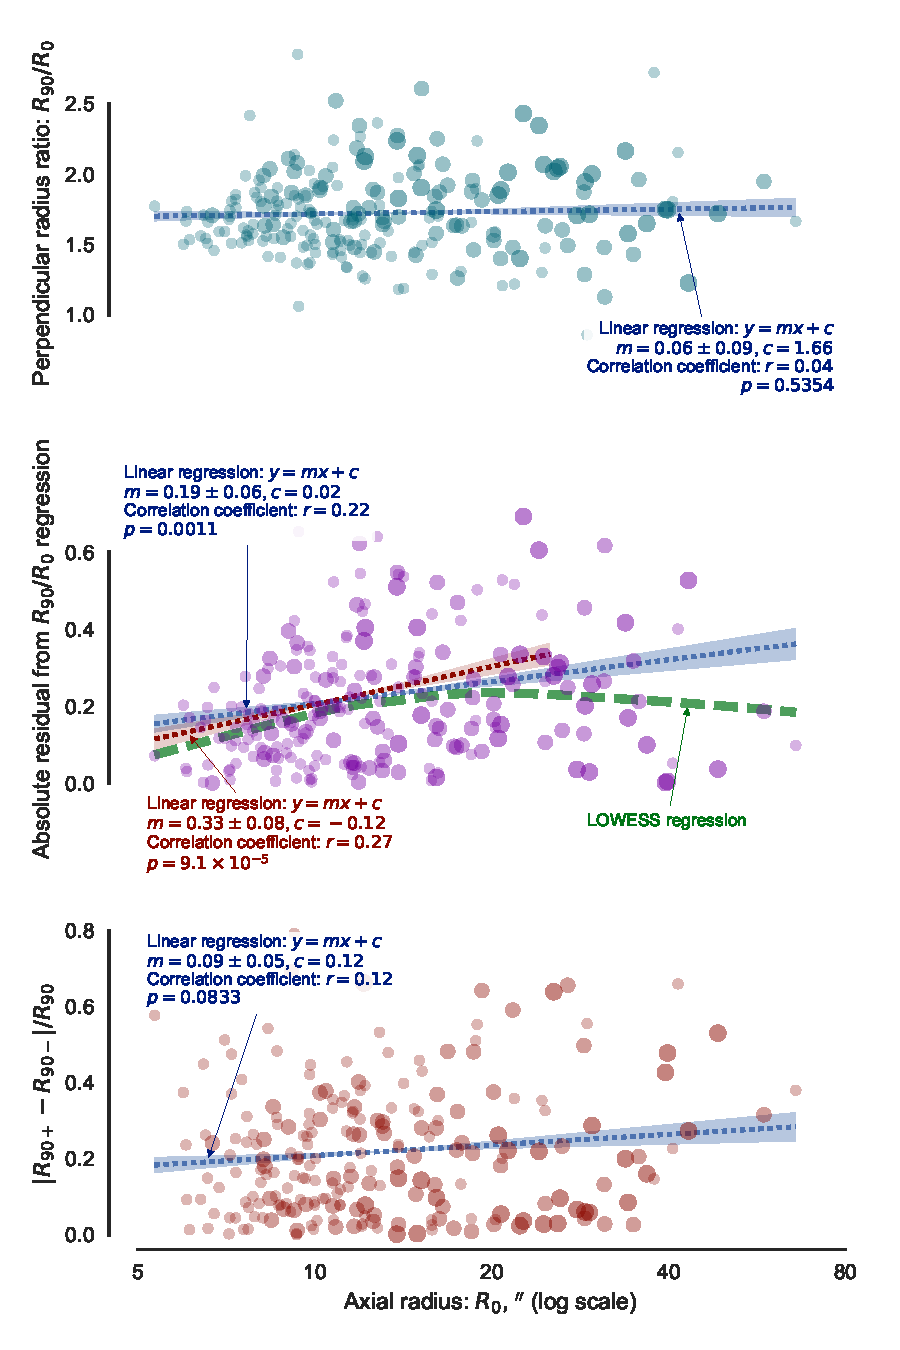
\includegraphics[width=\linewidth]{figs/mipsgal-R90-ratio-versus-R0-heteroscedastic}
  \caption{Regression analysis of bow shock wings shape versus size.
    The top panel shows a linear fit to \(R_{90}/R_0\) versus
    \(\log_{10} R_0\), which is essentially flat and is consistent
    with no correlation between the two quantities.  On the other
    hand, in the central panel, which shows the absolute values of the
    residuals from this fit, it is apparent that the dispersion about
    the average value of the bow shock shape parameter \(R_{90}/R_0\)
    increases with bow shock size.  A linear fit to all the data is
    shown by the blue dotted line, while a locally weighted regression
    (LOWESS; \citealp{Cleveland:1979a, Cleveland:1988a}) is shown by
    the heavy green dashed line.  The negative curvature of the LOWESS
    curve suggests that the slope of the linear fit is a compromise
    between a steeper slope for smaller bow shocks and a flat (or
    negative) slope for the largest bow shocks.  We therefore repeat
    the linear fit, but after excluding sources with \(R_0 > 25''\),
    with results shown by the red dotted line.  The bottom panel shows
    the bow shock wings asymmetry parameter,
    \(|R_{90+} - R_{90-}| / R_{90}\), together with a linear fit.
    Symbol size indicates the star rating of each source, from 3-star
    (smallest) to 5-star (largest).}
  \label{fig:mipsgal-heteroscedastic}
\end{figure}

We now investigate if the bow shock shapes of the MIPSGAL sources are
correlated with any other parameters via the following methodology:
\begin{enumerate}[1.]
\item For each of the parameters in the \citet{Kobulnicky:2016a}
  catalog, we divide the sources into two or more sub-samples,
  according to the value of the parameter.  For quantitative
  parameters, such as those discussed in the previous section, we use
  two sub-samples of equal size, with membership determined by whether
  the parameter is larger or smaller than the median value.  But we
  also use categorical parameters, such as the type of bow shock
  environment, or the presence/absence of \SI{8}{\um} emission, in
  which case the sub-samples are of unequal size.
\item We plot the KDEs of the two sub-samples separately on the
  \(R_c\)--\(R_{90}\) plane (see Figs.~\ref{fig:mipsgal-correlated} and
  \ref{fig:mipsgal-uncorrelated}) to check for any obvious
  differences.
\item We check if there is any statistically significant difference
  between the bow shock shapes of the sub-samples by applying three
  different non-parametric tests to \(R_c/R_0\) and \(R_{90}/R_0\)
  separately.  The principal test used is the two-sample
  Anderson--Darling test \citep{Anderson:1952a, Scholz:1987a,
    Makarov:2017a}, which is a general test of the \textit{null
    hypothesis} that the two sub-samples are drawn from the same
  distribution.  It returns a \(p\)-value, which is the estimated
  probability that the observed difference between the two sub-samples
  would be as large as it is purely by chance if they were all were
  drawn from the same distribution.  We consider two different
  thresholds for significance: \(p < 0.05\) (approximately
  2-\(\sigma\) for a normal distribution) and \(p < 0.003\) (approximately
  3-\(\sigma\)).  We show in Appendix~\ref{sec:distr-p-values} that the
  more stringent \(p < 0.003\) condition is required in order to
  confidently reject the null hypothesis and declare a ``significant''
  difference between the two sub-samples, but we also consider the
  less strict threshold of \(p < 0.05\) as an indicator of
  ``possible'' difference.  We supplement the general-purpose
  Anderson--Darling test with two tests that probe specific features of
  the sample distributions: the Mann--Whitney--Wilcoxon \(U\) test
  \citep{Mann:1947a}, which is sensitive to differences in the central
  value (e.g., median) and the Brown--Forsythe test
  \citep{Brown:1974a}, which is sensitive to differences in the
  variance, or width, of the distribution (see
  Appendix~\ref{sec:distr-p-values} for details).
\end{enumerate}

As shown in detail in Table~\ref{tab:big-p}, there is remarkably
little variation in the bow shock shape distributions as a function of
most of the other parameters.  Two examples in which there is
\textit{no} significant shape difference between the sub-samples are
shown in Figure~\ref{fig:mipsgal-uncorrelated}.  This lack of
difference is interesting because in both examples there are a priori
grounds to suspect that differences might exist.  The first example (Fig.~\ref{fig:mipsgal-uncorrelated}a) is
the bow shock environment, which was categorized in
\citet{Kobulnicky:2016a} as ``Isolated'' (I), ``Facing a large \hii{}
region'' (FH), ``Facing a \SI{8}{\um} bright-rimmed cloud'' (FB), and
``Within a giant \hii{} region'' (H), and where we have merged the FH
and FB categories, labelled ``Facing'' in the figure.\footnote{Similar
  results are also found for the FB and FH categories separately.}
The shapes might be expected to vary with environment because the FB
and FH categories should be associated with ``weather vane''
interactions \citep{Povich:2008a} between the stellar wind and a
divergent photoevaporation flow.  This is expected to give a more open
bow shock than in the ``runaway'' case of interaction of a moving star
with a static environment.  In the thin-shell approximation, the
predicted shapes are a carawilkinoid for weather vanes and a wilkinoid
for runaways, see \S~\ref{sec:crw-scenario}.  The fact that no such
difference is detected could be explained in one of two ways: (i)~the
momentum ratio \(\beta\) for the weather vanes could be small, since the
carawilkinoid becomes indistinguishable from the wilkinoid as
\(\beta \to 0\), or (ii)~many of the bow shocks classified as ``Isolated''
might also be weather vanes rather than runaways.

The second example (Fig.~\ref{fig:mipsgal-uncorrelated}b) divides the
sources according to whether or not \citet{Kobulnicky:2016a} judged
there to be multiple candidates for the identity of the central star
that drives the bow shock.  If the central star were to be
misidentified in a significant number of sources, then the measured
value of \(R_0\) for those sources would be erroneous, which would
increase the scatter in both \(R_c/R_0\) and \(R_{90}/R_0\).  The
fact that no significant difference is seen in the shape distributions
between sources with/without multiple candidates implies that such
mistakes in identification of the central star must be rare.

We also tested all the other source parameters listed in
\citeauthor{Kobulnicky:2016a}'s catalog, finding no significant shape
differences for sources with/without \SI{8}{\um} emission, with
low/high extinction, closer/farther from the Galactic plane, or
closer/farther from the Galactic center. Details are given in
Table~\ref{tab:big-p}.  In all these cases, differences in mean or
median \(R_{90}/R_0\) less than \(0.06\) and in \(R_c/R_0\) less than
\(0.16\) are found, corresponding to rank biserial correlation
coefficients (a non-parametric dimensionless measure of the difference
between two samples, see Appendix~\ref{sec:distr-p-values}) of
\(r_b < 0.15\), which are not significant even at the 2-\(\sigma\) level.

The only parameters that \emph{do} show a possible correlation with
the bowshock shape are the bow shock angular size, \(R_0\), and the
extinction-corrected magnitude of the central star, \(H_0\), which are
illustrated in Figure~\ref{fig:mipsgal-correlated}.  In both cases,
the general purpose Anderson--Darling test indicates differences in the
sub-sample distributions of \(R_{90} / R_0\) at the 2-\(\sigma\) level.  It
is apparent from the histograms shown in the right-hand inset graphs
of Figure~\ref{fig:mipsgal-correlated}a that in the case of the
small/large \(R_0\) sub-samples it is the width rather than the
central tendency of the distributions that is different, which is
confirmed by the more specific Brown--Forsythe test, which indicates a
difference between the sub-sample dispersions at the 3-\(\sigma\) level.
In the case of the faint/bright \(H_0\) sub-samples
(Fig.~\ref{fig:mipsgal-heteroscedastic}b), it is less clear what
feature of the distributions differ.

In order to investigate these effects in more detail and look for
systematic trends, we divide the independent parameter (\(R_0\) or
\(H_0\)) into 5 rather than 2 equal-sized sub-samples, with results
shown as box plots in Figure~\ref{fig:mipsgal-boxplot}.  A systematic
increase with \(R_0\) in the dispersion of \(R_{90}/R_0\) (upper panel
of Fig.~\ref{fig:mipsgal-boxplot}a) is apparent from both the
interquartile range (colored boxes) and interdecile range (error
bars).  As a check on whether observational uncertainties might be
contributing to this trend, the third and fourth rows of box plots
show the statistics for, respectively, the fractional asymmetry of the
bowshock wings and the standard deviation, \(\epsilon(R_{90})\), of the
individual points on the bow shock that go into determining \(R_{90}\)
(see step~\ref{step:R90} of the tracing/fitting methodology described
in \S~\ref{sec:autom-trac-fitt}).  It can be seen that neither of
these quantities tends to increase with \(R_0\), and in fact there is
a significant \emph{decrease} in \(\epsilon(R_{90})\) with \(R_0\).  This
implies that the increase with angular size of the diversity of bow
shock wing shapes is real, and not due to observational uncertainties.  
On the other hand, the fact that no clear trends are evident as a
function of source magnitude \(H_0\) (Fig.~\ref{fig:mipsgal-boxplot}b)
leads us to suspect that the \(p < 0.05\) result obtained for the
2-sample Anderson--Darling test was a \emph{false positive}, which is
also supported by the analysis in Appendix~\ref{sec:distr-p-values}
and Figure~\ref{fig:histo-p-values}.

So, the only correlation that survives scrutiny is the increase in
dispersion of \(R_{90}/R_0\) with increasing \(R_0\), which is finally
presented in the greatest detail in
Figure~\ref{fig:mipsgal-heteroscedastic}, where we eschew any binning
and perform linear regressions of the individual sources as a function
of \(\log_{10} R_0\).  As expected from the previous 2-sample and
5-sample analyses, the regression of \(R_{90}/R_0\) is almost flat,
with a low correlation coefficient, whereas a regression of the
absolute residuals to this fit against \(\log_{10} R_0\) shows a
significant positive slope.  This increase in dispersion of shape with
angular size is only evident for \(R_0 < 30''\), becoming flat at the
largest sizes (see middle panel of
Fig.~\ref{fig:mipsgal-heteroscedastic}).

As mentioned in \S~\ref{sec:ob-shapes} there is also a shape
difference between the 3-star sources and the 4/5-star sources (see
Fig.~\ref{fig:mipsgal-shapes}b).  The \(p\)-values of statistical
tests (see Table~\ref{tab:big-p}) indicate that this is much more
significant than any correlation with the other parameters discussed
in this section (\(p < 10^{-4}\) for \(R_{90}/R_0\) and
\(p < 10^{-5}\) for \(R_c/R_0\)).  This means that it cannot be simply
due to the tendency of the higher-rated sources to have larger angular
sizes.  However, the subjective nature of the star ratings makes this
result hard to interpret.

\subsection{Far-infrared arcs around late-type stars}
\label{sec:far-infrared-arcs}



\begin{figure*}
  \centering
  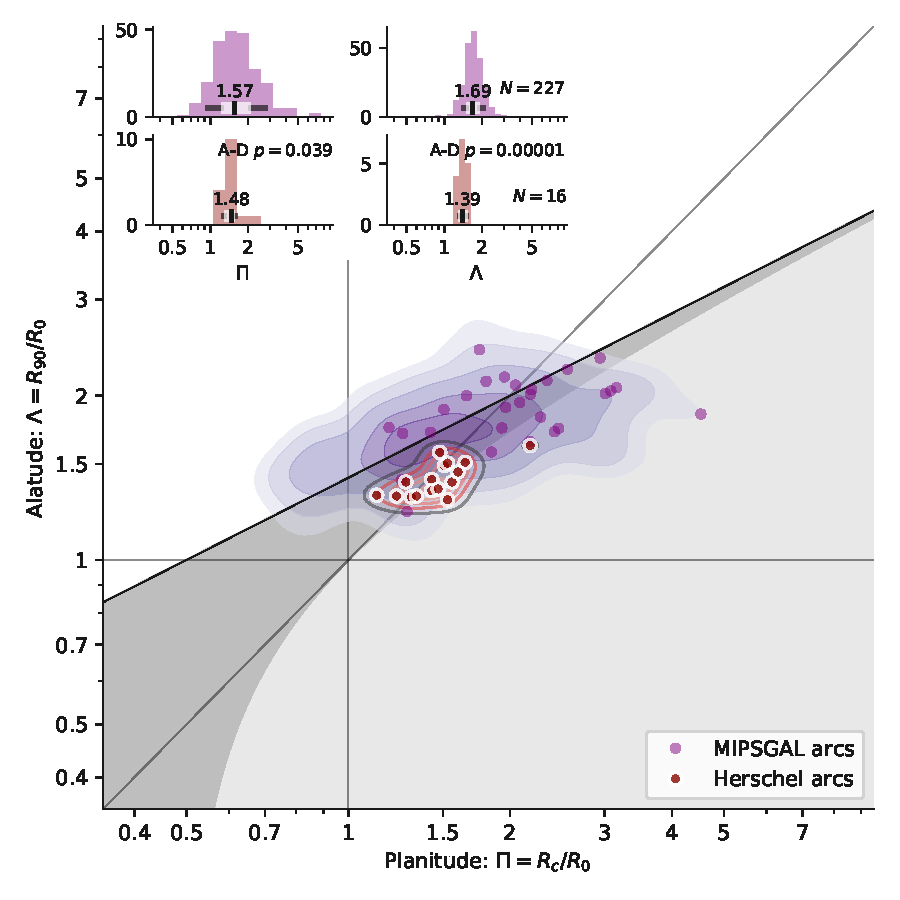
\includegraphics[width=\linewidth]{figs/mipsgal-Rc-R90-vs-Herschel}
  \caption[]{Comparison of RSG/AGB arcs with OB star arcs.}
  \label{fig:herschel-compare-mipsgal}
\end{figure*}



\subsection{Stationary emission line arcs in M42}
\label{sec:stat-emiss-line}

\begin{figure*}
  \centering
  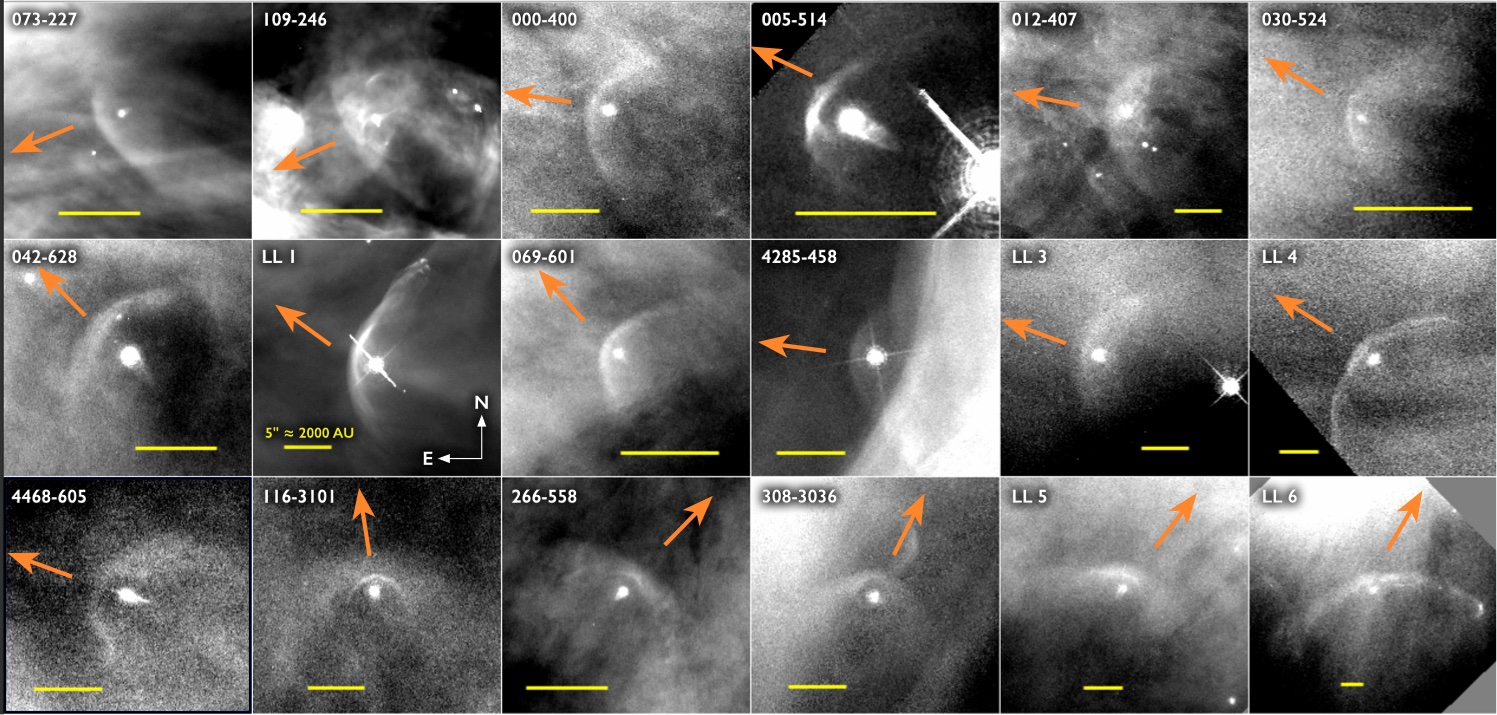
\includegraphics[width=\textwidth]{figs/annotated-ll-arcs}
  \caption[]{Stationary bow shock arcs in the Orion Nebula.}
  \label{fig:ll-arcs}
\end{figure*}

\begin{figure*}
  \centering
  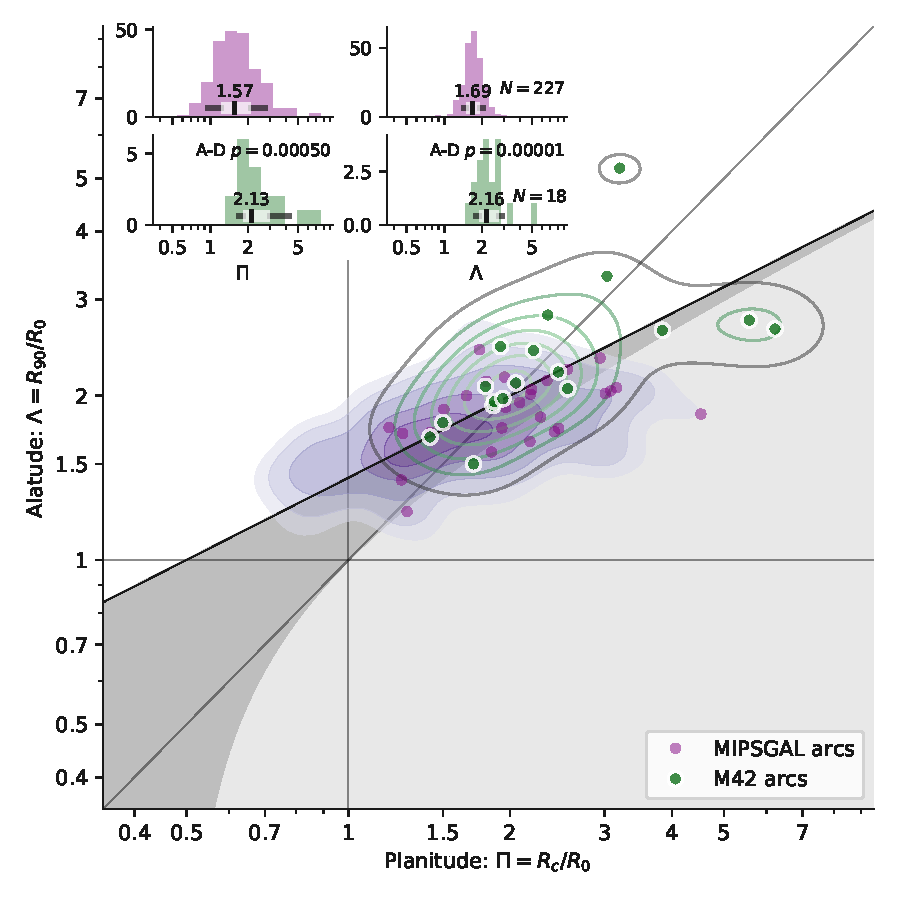
\includegraphics[width=\linewidth]{figs/mipsgal-Rc-R90-vs-Orion}
  \caption[]{Comparison of Orion with OB stars.}
  \label{fig:ll-compare-mipsgal}
\end{figure*}


Mention future JWST observations with \(0.85\arcsec\) resolution at \SI{22}{\um}. 


%%% Local Variables:
%%% mode: latex
%%% TeX-master: "quadrics-bowshock.tex"
%%% End:

\section{Perturbed bows}
\label{sec:perturbed-bows}

\begin{figure*}
  \centering
  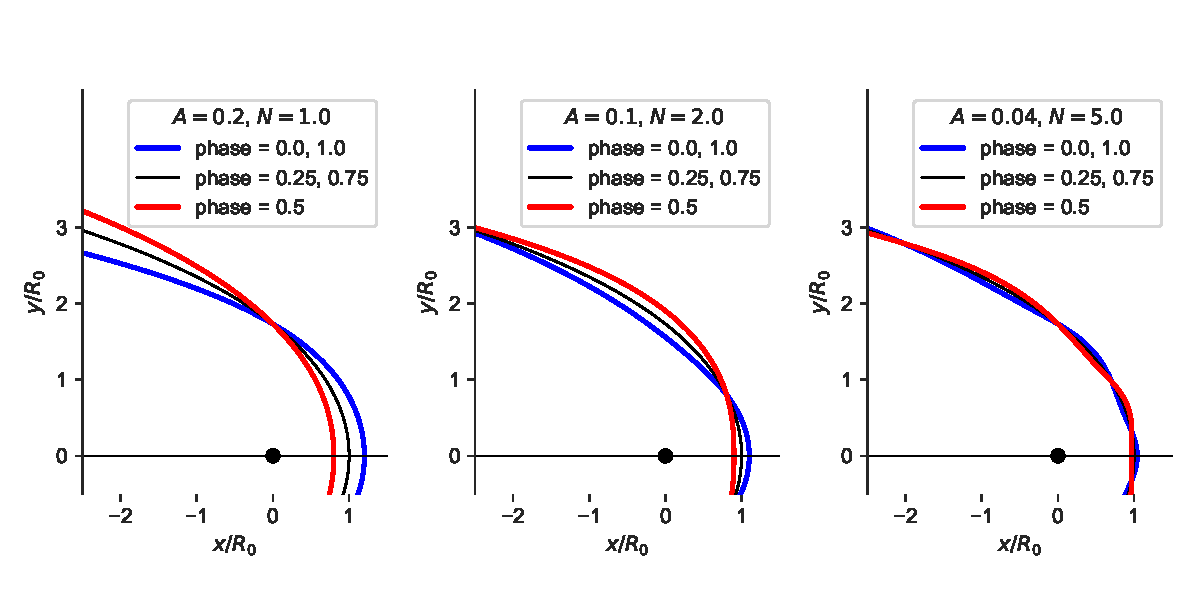
\includegraphics[width=\linewidth]{figs/compare_xyprime_wave-wilkinoid}
  \caption{Small-amplitude standing wave perturbations to bow shapes.}
  \label{fig:perturb-shapes}
\end{figure*}

\begin{figure*}
  \centering
  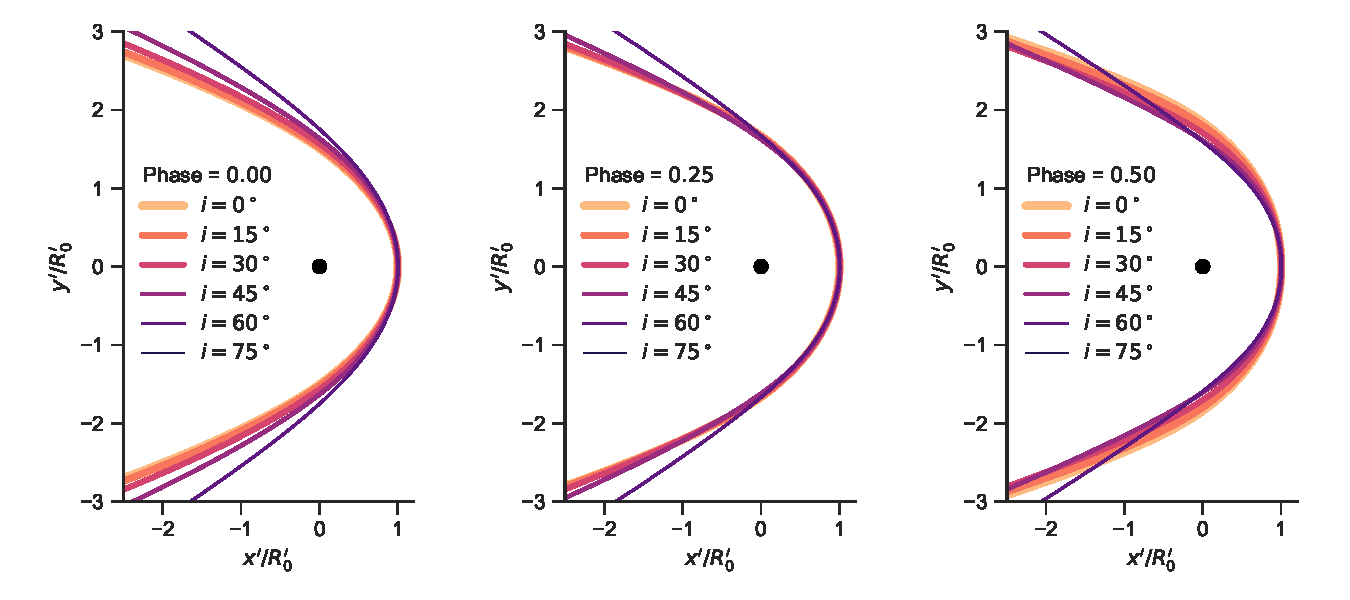
\includegraphics[width=\linewidth]
  {figs/wave_xyprime-A005-N20-ancantoid-xi080-beta000500}
  \caption{Plane-of-sky projections of perturbed bow shapes}
  \label{fig:perturb-xy-prime}
\end{figure*}

The bow shock models that we have considered so far have been
steady-state: although material is moving throughout the bow, the
pattern of its structure does not vary with time.  In this section, we
consider small, time-varying perturbations to such a steady-state
structure.  These may be due to periodic variations in the
momentum-loss rate of one of the winds, or due to dynamical
instabilities in the shocked shell.

For simplicity, we consider standing waves with an amplitude that
multiplies the bow shock radius \(R\) and a pattern that is periodic
in the axial angle \(\theta\): \(R(\theta) \to (1 + \Delta) R(\theta)\), where
\begin{equation}
  \label{eq:standing-wave}
  \Delta = A \cos(N \theta) \cos(2\pi \varphi)
\end{equation}

\begin{figure}
  \centering
  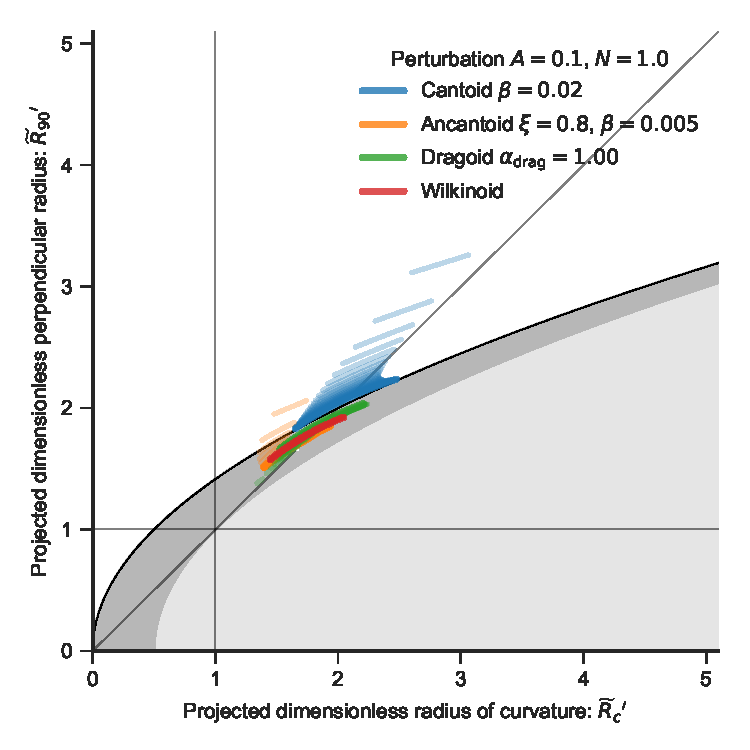
\includegraphics[width=\linewidth]
  {figs/wave-R90-vs-Rc-A010-N10}
  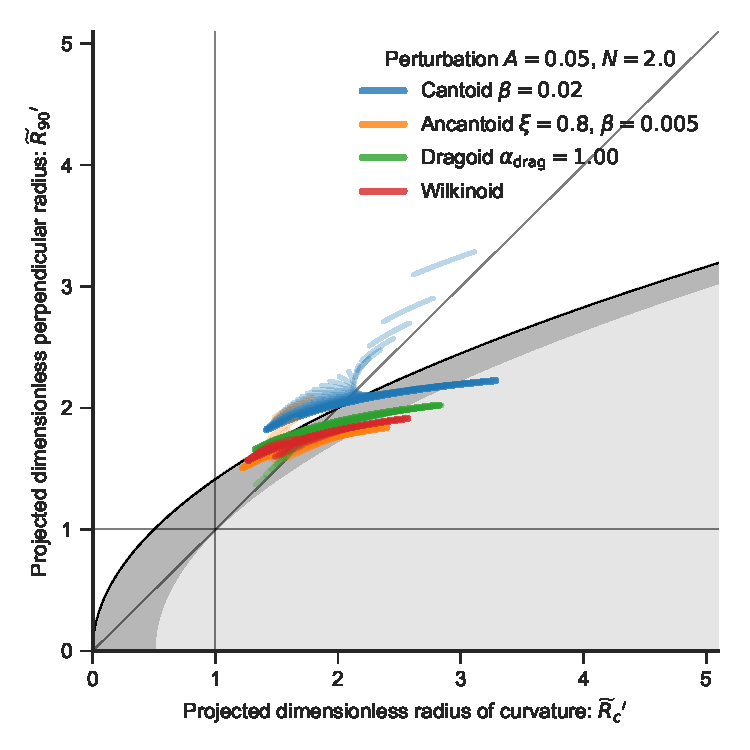
\includegraphics[width=\linewidth]
  {figs/wave-R90-vs-Rc-A005-N20}
  \caption{Diagnostic diagram for perturbed shapes}
  \label{fig:perturb-Rc-R90}
\end{figure}


%%% Local Variables:
%%% mode: latex
%%% TeX-master: "quadrics-bowshock"
%%% End:


\section{Conclusions}
\label{sec:conclusion}

Difference in SEDs between FIR and MIR samples?  \citet{Meyer:2016a}
say emission peaks at 3--50 micron for O star bow shocks.

Al other things being equal, larger bows will be at higher
inclinations (we should estimate how much variation in size we should
get due to inclination -- it will be more for flatter bows).  Higher
inclinations means less variation from the standing wave oscillations,
which goes against our result that larger bows have greater dispersion
in \(\Lambda'\).  Although the standing waves mainly give dispersion in
\(\Pi'\) anyhow.

%%% Local Variables:
%%% mode: latex
%%% TeX-master: "obs-bowshocks"
%%% End:

\clearpage
\bibliographystyle{mnras}
%% All references should be put in the BibTeX file bowshocks-biblio.bib
\bibliography{bowshocks-biblio}
\appendix

\section{Distribution of p-values for all correlations tested}
\label{sec:distr-p-values}

\begin{figure}
  (a)\\
  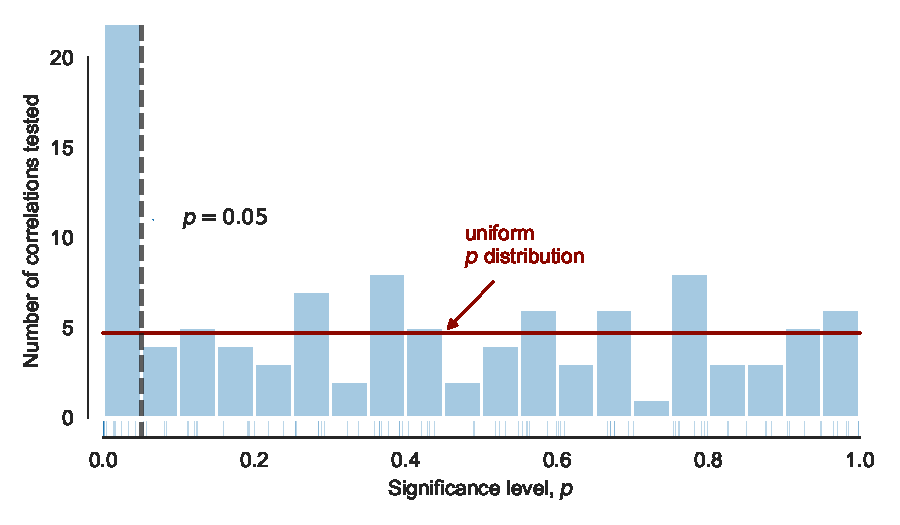
\includegraphics[width=\linewidth]{figs/p-value-histogram-new-linear}\\
  (b)\\
  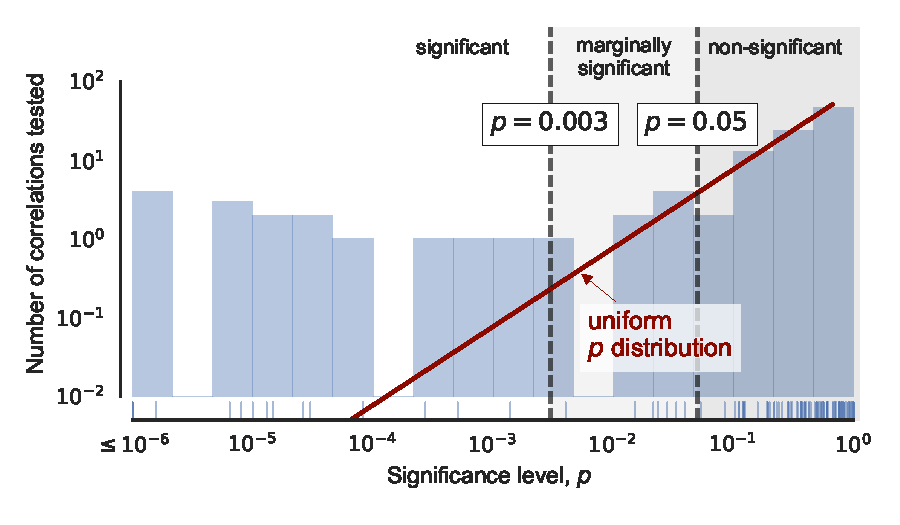
\includegraphics[width=\linewidth]{figs/p-value-histogram-new}
  \caption{Histogram of \(p\)-values for all non-parametric 2-sample
    tests listed in Table~\ref{tab:big-p}. (a)~Uniformly spaced linear
    bins and linear vertical axis. (b)~Uniformly spaced logarithmic
    bins and logarithmic vertical axis, with all values
    \(p \le 10^{-6}\) included in the leftmost bin.  Short thin vertical
    lines above the horizontal axis show the individual values.  The
    thick vertical dashed lines show the traditional threshold values
    for significance: \(p = 0.003\) (\(\approx 3 \sigma\)) and
    \(p = 0.05\) (\(\approx 2 \sigma\)). The red solid line shows the uniform
    distribution of \(p\)-values that would be expected if the null
    hypothesis were always true, that is, if no significant
    correlations existed.}
  \label{fig:histo-p-values}
\end{figure}

\begin{table*}
  \sisetup{detect-all=true, detect-inline-weight=math}
  \sisetup{round-mode=figures, round-precision=2}
  \sisetup{table-align-exponent = false}
  \setlength\tabcolsep{2pt}
  \caption{Results of all statistical tests performed on observed bow
    shock shape parameters. Significant correlations are shown in
    \textbf{bold}, marginally significant correlations in
    \textit{italic}}
  \label{tab:big-p}
  %%% MIPSGAL summary statistics
%%% Table automatically generated from mipsgal-summary-stats.tab
%%% 2017-06-08 14:17:39.847703
%%%
% \Width is used to align number under col header in first column
	\newlength\Width\settowidth\Width{Comparison}
	\begin{tabular}{@{} ll @{\quad } S[round-mode=places]S[round-mode=places] S[round-mode=places]S[round-mode=places] SS SS @{\quad\quad\quad} SSS[round-mode=places] @{\quad} S@{}S@{}S @{}}\toprule
	  & {Dependent} & \multicolumn{2}{c}{Mean} & \multicolumn{2}{c}{Std.\ Dev.} & \multicolumn{2}{c}{Obs.\ Disp.} & \multicolumn{2}{c @{\quad\quad\quad}}{s.e.m.} & \multicolumn{3}{c @{\quad} }{\dotfill Effect sizes\dotfill } & \multicolumn{3}{c}{\dotfill Non-parametric test \(p\)-values  \dotfill} \\ 
	  {Comparison} & {Variable} & {\(\langle \text{A} \rangle\)} & {\(\langle \text{B} \rangle\)} & {\(\sigma_{\text{A}}\)} & {\(\sigma_{\text{B}}\)} & {\(\langle \epsilon_{\text{A}} \rangle\)} & {\(\langle \epsilon_{\text{B}} \rangle\)} & {\((\sigma/\!\sqrt n)_{\text{A}}\)} & {\((\sigma/\!\sqrt n)_{\text{B}}\)} & {\(r_b\)} & {Cohen \(d\)} & {\(\sigma_{\text{A}}/\sigma_{\text{B}}\)} & \multicolumn{1}{c}{Anderson--Darling} & \multicolumn{1}{c}{Rank biserial} &  \multicolumn{1}{c}{Brown--Forsythe}\\
	  {\makebox[\Width]{(1)}} & \multicolumn{1}{c@{\quad}}{(2)} & {(3)} & {(4)} & {(5)} & {(6)} & {(7)} & {(8)} & {(9)} & {(10)}  & {(11)} & {(12)} & {(13)} & {(14)} & {(15)} & {(16)} \\  
	  \midrule\multicolumn{10}{@{} l @{\quad\quad\quad}}{\itshape Median split of continuous independent variables \dotfill}\\
\addlinespace
Faint/bright & \(R_{90} / R_{0}\) & 1.677 & 1.768 & 0.269 & 0.316 & 0.231 & 0.236 & 0.025 & 0.03 & \itshape 0.174 & \itshape 0.308 & 1.175 & \itshape 0.0215 & \itshape 0.0235 & 0.125\\
\(H\) magnitude & \(\Delta R_{90} / R_{90}\) & 0.183 & 0.198 & 0.161 & 0.163 &   &   & 0.015 & 0.015 & 0.07 & 0.093 & 1.013 & 0.538 & 0.365 & 0.761\\
\(n_{\text{A}} =  n_{\text{B}} = 113\) & \(R_{c} / R_{0}\) & 1.655 & 1.917 & 0.631 & 1.045 & 0.097 & 0.078 & 0.059 & 0.098 & 0.123 & 0.303 & \itshape 1.654 & 0.123 & 0.111 & \itshape 0.0335\\
\addlinespace
Low/high & \(R_{90} / R_{0}\) & 1.707 & 1.739 & 0.25 & 0.336 & 0.256 & 0.212 & 0.024 & 0.031 & 0.061 & 0.11 & \bfseries 1.342 & \itshape 0.0281 & 0.428 & \bfseries 0.00139\\
bow shock size, \(R_0\) & \(\Delta R_{90} / R_{90}\) & 0.175 & 0.204 & 0.157 & 0.165 &   &   & 0.015 & 0.015 & 0.091 & 0.176 & 1.054 & 0.103 & 0.238 & 0.193\\
\(n_{\text{A}} =  n_{\text{B}} = 113\) & \(R_{c} / R_{0}\) & 1.766 & 1.803 & 0.975 & 0.755 & 0.114 & 0.062 & 0.092 & 0.071 & 0.1 & 0.043 & 0.774 & 0.228 & 0.192 & 0.599\\
\addlinespace
Low/high & \(R_{90} / R_{0}\) & 1.703 & 1.742 & 0.267 & 0.323 & 0.233 & 0.235 & 0.025 & 0.03 & 0.04 & 0.132 & 1.213 & 0.554 & 0.602 & 0.123\\
extinction, \(A_K\) & \(\Delta R_{90} / R_{90}\) & 0.186 & 0.195 & 0.138 & 0.183 &   &   & 0.013 & 0.017 & -0.039 & 0.057 & 1.326 & 0.301 & 0.61 & 0.112\\
\(n_{\text{A}} =  n_{\text{B}} = 113\) & \(R_{c} / R_{0}\) & 1.725 & 1.846 & 0.822 & 0.917 & 0.091 & 0.085 & 0.077 & 0.086 & 0.082 & 0.139 & 1.116 & 0.219 & 0.285 & 0.982\\
\addlinespace
Low/high & \(R_{90} / R_{0}\) & 1.722 & 1.724 & 0.328 & 0.261 & 0.234 & 0.234 & 0.031 & 0.024 & 0.02 & 0.008 & 0.796 & 0.308 & 0.795 & 0.0534\\
\(\vert{}b\vert\) & \(\Delta R_{90} / R_{90}\) & 0.188 & 0.191 & 0.161 & 0.162 &   &   & 0.015 & 0.015 & 0.009 & 0.021 & 1.005 & 0.964 & 0.907 & 0.694\\
\(n_{\text{A}} =  n_{\text{B}} = 113\) & \(R_{c} / R_{0}\) & 1.706 & 1.862 & 0.727 & 0.988 & 0.085 & 0.091 & 0.068 & 0.092 & 0.069 & 0.181 & 1.358 & 0.19 & 0.368 & 0.0842\\
\addlinespace
High/low & \(R_{90} / R_{0}\) & 1.734 & 1.707 & 0.279 & 0.321 & 0.241 & 0.223 & 0.024 & 0.034 & -0.049 & -0.093 & 1.152 & 0.361 & 0.532 & 0.159\\
\(\cos \ell\) & \(\Delta R_{90} / R_{90}\) & 0.182 & 0.201 & 0.155 & 0.171 &   &   & 0.013 & 0.018 & 0.054 & 0.122 & 1.1 & 0.604 & 0.491 & 0.365\\
\(n_{\text{A}}, n_{\text{B}} = 137, 90\) & \(R_{c} / R_{0}\) & 1.807 & 1.751 & 0.946 & 0.742 & 0.09 & 0.084 & 0.081 & 0.078 & -0.0 & -0.064 & 0.785 & 1.03 & 0.999 & 0.549\\
\midrule
\multicolumn{10}{@{} l @{\quad\quad\quad}}{\itshape Categorical independent variables \dotfill}\\
\addlinespace
Environment: & \(R_{90} / R_{0}\) & 1.735 & 1.693 & 0.283 & 0.338 & 0.238 & 0.218 & 0.022 & 0.053 & -0.07 & -0.142 & 1.194 & 0.603 & 0.49 & 0.392\\
Isolated vs Facing & \(\Delta R_{90} / R_{90}\) & 0.19 & 0.195 & 0.161 & 0.172 &   &   & 0.012 & 0.027 & -0.019 & 0.034 & 1.066 & 0.507 & 0.85 & 0.438\\
\(n_{\text{A}}, n_{\text{B}} = 170, 41\) & \(R_{c} / R_{0}\) & 1.757 & 1.852 & 0.854 & 0.899 & 0.087 & 0.083 & 0.066 & 0.14 & 0.042 & 0.11 & 1.053 & 0.713 & 0.676 & 0.377\\
\addlinespace
Environment: & \(R_{90} / R_{0}\) & 1.735 & 1.68 & 0.283 & 0.309 & 0.238 & 0.233 & 0.022 & 0.077 & -0.13 & -0.193 & 1.092 & 0.518 & 0.391 & 0.782\\
Isolated vs \hii & \(\Delta R_{90} / R_{90}\) & 0.19 & 0.175 & 0.161 & 0.138 &   &   & 0.012 & 0.034 & -0.048 & -0.095 & 0.855 & 0.932 & 0.754 & 0.799\\
\(n_{\text{A}}, n_{\text{B}} = 170, 16\) & \(R_{c} / R_{0}\) & 1.757 & 1.907 & 0.854 & 0.955 & 0.087 & 0.105 & 0.066 & 0.239 & 0.024 & 0.174 & 1.118 & 0.496 & 0.875 & 0.255\\
\addlinespace
Single/multiple & \(R_{90} / R_{0}\) & 1.709 & 1.762 & 0.289 & 0.315 & 0.23 & 0.243 & 0.022 & 0.041 & 0.074 & 0.177 & 1.09 & 0.342 & 0.396 & 0.338\\
source candidate & \(\Delta R_{90} / R_{90}\) & 0.184 & 0.206 & 0.162 & 0.16 &   &   & 0.013 & 0.021 & 0.093 & 0.136 & 0.987 & 0.421 & 0.284 & 0.97\\
\(n_{\text{A}}, n_{\text{B}} = 167, 60\) & \(R_{c} / R_{0}\) & 1.767 & 1.833 & 0.825 & 0.988 & 0.09 & 0.08 & 0.064 & 0.128 & 0.027 & 0.076 & 1.198 & 0.999 & 0.756 & 0.605\\
\addlinespace
With/without & \(R_{90} / R_{0}\) & 1.734 & 1.721 & 0.289 & 0.298 & 0.223 & 0.237 & 0.043 & 0.022 & -0.042 & -0.044 & 1.031 & 0.595 & 0.667 & 0.563\\
\SI{8}{\um} emission & \(\Delta R_{90} / R_{90}\) & 0.203 & 0.186 & 0.205 & 0.149 &   &   & 0.031 & 0.011 & 0.021 & -0.106 & 0.726 & 0.765 & 0.826 & 0.219\\
\(n_{\text{A}}, n_{\text{B}} = 45, 182\) & \(R_{c} / R_{0}\) & 1.714 & 1.802 & 0.598 & 0.926 & 0.091 & 0.087 & 0.089 & 0.069 & -0.012 & 0.101 & 1.547 & 0.824 & 0.904 & 0.2\\
\addlinespace
3-star vs (4+5)-star & \(R_{90} / R_{0}\) & 1.661 & 1.812 & 0.288 & 0.286 & 0.247 & 0.216 & 0.025 & 0.029 & \bfseries 0.328 & \bfseries 0.525 & 0.99 & \bfseries 8.23e-05 & \bfseries 2.63e-05 & 0.403\\
 & \(\Delta R_{90} / R_{90}\) & 0.189 & 0.19 & 0.162 & 0.161 &   &   & 0.014 & 0.017 & -0.007 & 0.009 & 0.994 & 0.809 & 0.927 & 0.561\\
\(n_{\text{A}}, n_{\text{B}} = 133, 94\) & \(R_{c} / R_{0}\) & 1.632 & 2.0 & 0.91 & 0.764 & 0.106 & 0.061 & 0.079 & 0.079 & \bfseries 0.386 & \bfseries 0.431 & 0.84 & \bfseries 1.47e-05 & \bfseries 7.66e-07 & 0.762\\
\midrule
\multicolumn{10}{@{} l @{\quad\quad\quad}}{\itshape Intercomparison with other datasets \dotfill}\\
\addlinespace
MIPS vs Orion & \(R_{90} / R_{0}\) & 1.723 & 2.418 & 0.297 & 0.811 &   &   & 0.02 & 0.191 & \bfseries 0.7 & \bfseries 1.928 & \bfseries 2.735 & \bfseries 8.02e-06 & \bfseries 7.84e-07 & \bfseries 6.41e-06\\
 & \(\Delta R_{90} / R_{90}\) & 0.19 & 0.701 & 0.162 & 0.532 &   &   & 0.011 & 0.148 & \bfseries 0.689 & \bfseries 2.553 & \bfseries 3.29 & \bfseries 9.94e-06 & \bfseries 3e-05 & \bfseries 2.42e-10\\
\(n_{\text{A}}, n_{\text{B}} = 227, 18\) & \(R_{c} / R_{0}\) & 1.784 & 2.639 & 0.871 & 1.302 &   &   & 0.058 & 0.307 & \bfseries 0.516 & \bfseries 0.94 & 1.495 & \bfseries 0.000505 & \bfseries 0.000273 & 0.12\\
\addlinespace
MIPS vs RSG & \(R_{90} / R_{0}\) & 1.723 & 1.402 & 0.297 & 0.092 &   &   & 0.02 & 0.035 & \bfseries -0.742 & \bfseries -1.098 & \itshape 0.311 & \bfseries 0.000571 & \bfseries 0.000841 & \itshape 0.0406\\
 & \(\Delta R_{90} / R_{90}\) & 0.19 & 0.15 & 0.162 & 0.087 &   &   & 0.011 & 0.033 & -0.072 & -0.247 & 0.539 & 0.795 & 0.747 & 0.286\\
\(n_{\text{A}}, n_{\text{B}} = 227, 7\) & \(R_{c} / R_{0}\) & 1.784 & 1.437 & 0.871 & 0.083 &   &   & 0.058 & 0.031 & -0.191 & -0.405 & 0.095 & 0.0798 & 0.392 & 0.053
\\
\bottomrule
\end{tabular}

\end{table*}

Results from all the statistical tests of the shape distributions
discussed in \S~\ref{sec:corr-shape} are given in
Table~\ref{tab:big-p}.  The \(p\)-values are the probability of
finding a difference between two populations at least as large as what
is observed \emph{given} that there is no difference in the underlying
distribution from which the two populations are drawn (that is, given
that the null hypothesis is true).  Conventionally, the null
hypothesis is rejected at a certain significance threshold \(\alpha\) when
\(p < \alpha\).  Since we are blindly testing many different hypotheses at
once, the commonly used \(\alpha = 0.05\) threshold is too lenient.  In
Figure~\ref{fig:histo-p-values} we analyse the frequency distribution
of \(p\) from all our tests \citep[see][]{Head:2015a}, finding a
systematic excess over a uniform distribution only for \(p < 0.01\).
We therefore take \(\alpha = 0.003\) as the optimum threshold in order to
balance the risks of false positives and false negatives. A false
positive is the erroneous rejection of the null hypothesis (the
spurious detection of a correlation that is not really there), while a
false negative is failing to detect a true correlation.


% However, what we really want to
% know is something else: the probability that the null hypothesis is
% true, \emph{given} the observations.  That is, the probability,
% \(\alpha\), of a \textit{false positive}, also known as the \textit{Type I
%   error rate}.  The common mistake of conflating these two definitions
% is known as the ``\(p\)-value fallacy'' \citep{Goodman:1999a}, or``the
% error of the transposed conditional'', as discussed in detail by
% \citet{Colquhoun:2014a}.  It is possible to derive \(\alpha\) from
% \(p\) using Bayes' theorem (e.g., \citealp{Goodman:1999b}), but that
% requires an estimate of the prior probability of the null hypothesis,
% independent of the observations.  Alternatively, it is also possible
% to find a lower bound on \(\alpha\) from a frequentist approach
% \citep{Sellke:2001a}:
% \begin{equation}
%   \label{eq:type-I}
%   \alpha(p) \ge \bigg[ 1 - \big(e\, p \ln p\big)^{-1} \bigg]^{-1}
%   \quad \text{valid for } p < 1/e.
% \end{equation}
% This is the approach we adopt here, which also numerically coincides
% with the Bayesian approach for the case where the prior probability of
% the null hypothesis is 0.5.  The reason that this is only a lower
% limit for \(\alpha\) is that if we have overwhelming a priori evidence that
% the null hypothesis is true (for instance, from previous empirical
% studies, or because it follows from a well-supported theory), then a
% Bayesian calculation would give a much higher value of \(\alpha\) than
% \eqref{eq:type-I} does.  In our case, however, we have no strong
% reasons for favoring any of the null hypotheses, so it is reasonable
% to assume \(\alpha\) is close to the lower limit given in \eqref{eq:type-I}.

% In order to choose a threshold \(p\)-value that counts as a
% ``significant'' result, one then needs to balance the risks of false
% positives against the risks of \textit{false negatives}.  The false
% negative probability, \(\beta\), also known as \textit{Type II error
%   rate}, is the probability of failing to reject an untrue null
% hypothesis.  That is, in the context of this paper, it is the
% probability of failing to detect a real difference between two
% sub-samples, or a real correlation between two variables.  The
% complementary probability, \(1 - \beta\), is known as the
% \textit{statistical power} or sensitivity of the test.  The value of
% \(\beta\) depends on three factors:
% \begin{enumerate}[1.]
% \item The \textit{effect size}, which is a measure of the magnitude of
%   the difference in a dependent variable between two sub-samples, or
%   the degree of correlation between two continuous variables.  For the
%   two sub-sample case, it is common to use a standardised mean
%   difference, such as Cohen's \(d\) statistic \citep{Cohen:1988a}:
%   \(d = (\bar{X}_A - \bar{X}_B) / s\), where \(\bar{X}_A\),
%   \(\bar{X}_B\) are the means of the dependent variable \(X\) for
%   samples A and B, while \(s\) is the pooled standard deviation of
%   \(X\).  For the case of two continuous variables, the Pearson linear
%   correlation coefficient, \(r\), can be used.  In both cases, rules
%   of thumb have been developed \citep{Ruscio:2008a} for classifying an
%   effect as ``large'' (\(d > 0.8\), \(r > 0.4\)) or ``small''
%   (\(d < 0.2\), \(r < 0.1\)).  Alternatively, non-parametric
%   statistics can be used, such as the \(A\) measure of stochastic
%   superiority \citep{Delaney:2002a}.
% \end{enumerate}

% Obviously, this depends on the \textit{effect size}, which is the 


% All astronomical data analysis is \emph{post hoc} analysis, since the universe was not set up to test a particular hypothesis (as far as we know).  It is therefore important to guard against the ``multiple comparisons problem'', whereby seemingly significant correlations are found where none really exist, simply by virtue of the large number of tests that were carried out.

% Under the more conservative Holm--Bonferroni method, only comparisons with \(p < 0.001\) would be significant. 

% The p-curve \citep{Head:2015a}

% \begin{table}
%   \caption{Results of all statistical tests performed on observed
%     bow shock shape parameters.}
%   \begin{tabular}{p{0.95\linewidth}}
%     \toprule
%     \textit{Description of columns:}
%     (Col.~1)~How the two A/B source sub-samples are defined, also giving the size of each sub-sample, \(n_{\text{A}}\) and~\(n_{\text{B}}\).
%     (Col.~2)~Dependent variable whose distribution is compared between the two sub-samples.
%     (Cols.~3--6)~Mean and standard deviation, \(\sigma\), of the dependent variable for each of the two sub-samples.
%     (Cols.~7--8)~Mean over each sub-sample of the observational dispersion (\(\epsilon\), standard deviation) of radii that contribute to the dependent variable for each individual source, as in steps~\ref{step:R0} and \ref{step:R90} of \S~\ref{sec:autom-trac-fitt}.  Note that in the case of \(R_c\), this is \(\epsilon(R_0)\), and so is not a direct measure of the observational uncertainty in \(R_c\). 
%     (Cols.~9--10)~``Standard error of the mean'' (s.e.m.) of the dependent variable for each of the two sub-samples. 
%     (Cols.~11--13)~Standardized ``effect sizes'', which are dimensionless measures of the difference in the distribution of the dependent variable between the two sub-samples.
%     (Col.~11)~Rank biserial correlation coefficient \citep{Cureton:1956a}, which is obtained by considering all \(n_{\text{A}} n_{\text{B}}\) pair-wise comparisons of the dependent variable between a source in sub-sample~A and a source in sub-sample~B.  It is the difference between the fraction of such comparisons ``won'' by sub-sample~A and those ``won'' by sub-sample~B, and thus may vary between \(-1\) and \(+1\). 
%     (Col.~12)~Cohen's \(d\), which is a dimensionless mean difference: \(d = (\langle \text{A} \rangle - \langle \text{B} \rangle) / \sigma_{\text{pool}} \), where \(\sigma_{\text{pool}} = (n_{\text{A}} \sigma_{\text{A}}^2 + n_{\text{B}} \sigma_{\text{B}}^2)^{1/2} / \sqrt{n_{\text{A}} + n_{\text{B}}}\) is the pooled standard deviation.
%     (Col.~13)~Ratio of standard deviations between the two sub-samples.
%     (Cols.~14--16)~Probabilities (\(p\)-values) of the two sub-samples being as different as observed if they were to be drawn from the same population, according to three different non-parametric tests.
%     (Col.~14)~Anderson--Darling 2-sample test, which is a general test of similarity between two distributions that is designed to retain sensitivity to differences in the tails of the distributions.
%     (Col.~15)~Mann--Whitney--Wilcoxon \(U\) test \citep{Mann:1947a}, which is sensitive to differences in the central value of the distributions.
%     (Col.~16)~Brown--Forsythe test for equality of variance \citep{Brown:1974a}
%     \\
%     \bottomrule
%   \end{tabular}
% \end{table}





\section{Perturbed bow shocks}
\label{sec:perturbed-bows}

\begin{figure*}
  \centering
  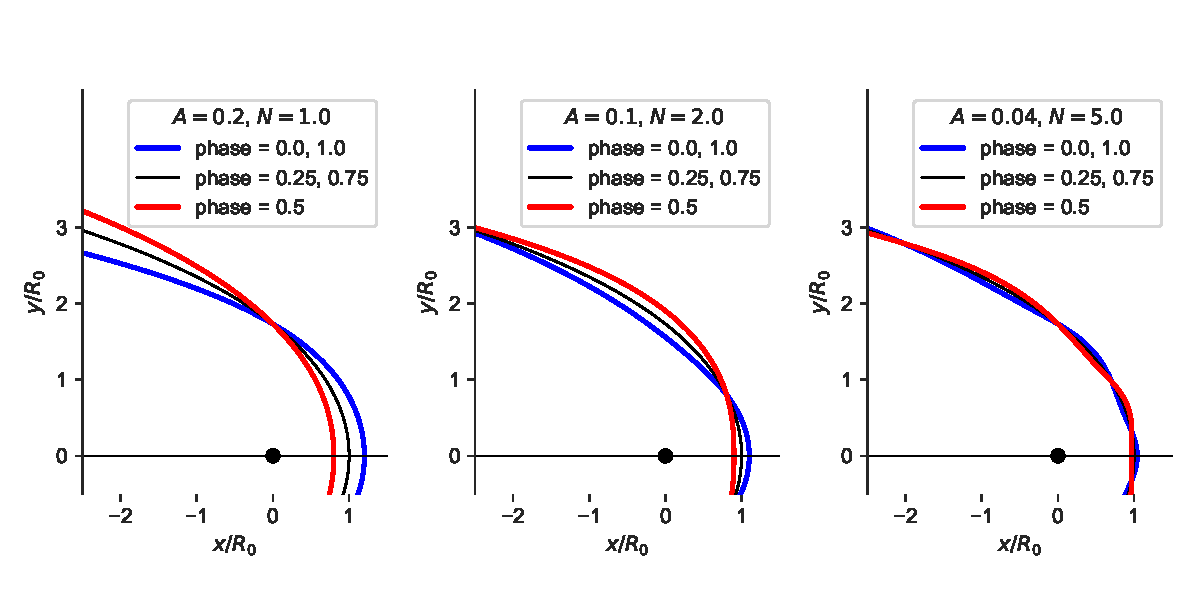
\includegraphics[width=\linewidth]{figs/compare_xyprime_wave-wilkinoid}
  \caption{Small-amplitude standing wave perturbations to wilkinoid
    bow shapes.  The maximum deviations from the base shape are seen
    at phases \(\phi = 0\) (blue line) and \(\phi = 0.5\) (red line), while
    the perturbation is zero at \(\phi = 0.25\) and \(0.75\) (black
    line).  Results are shown left to right for increasing wave
    numbers \(N\) and decreasing amplitudes \(A\): (a)~\(A = 0.2\),
    \(N = 1.0\), (b)~\(A = 0.1\), \(N = 2.0\), (a)~\(A = 0.04\),
    \(N = 5.0\).  The maximum curvature, proportional to \(A N\) is
    the same in all three cases.}
  \label{fig:perturb-shapes}
\end{figure*}
\begin{figure*}
  \centering
  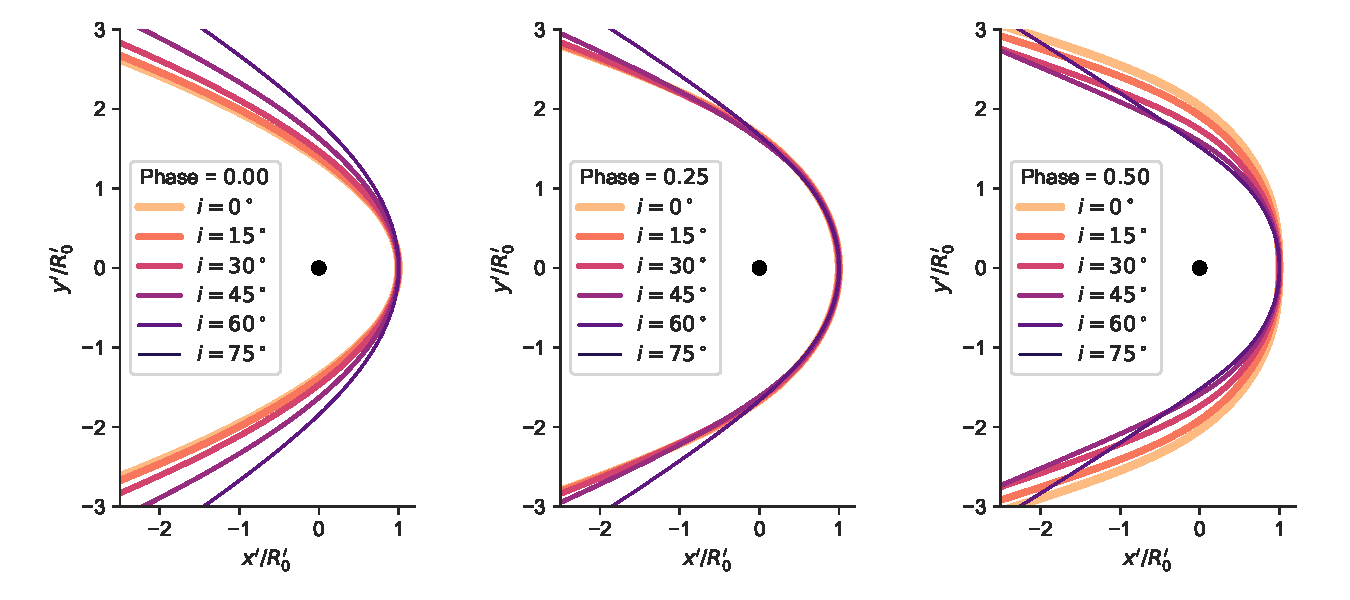
\includegraphics[width=\linewidth]
  {figs/wave_xyprime-A010-N20-ancantoid-xi080-beta000500}
  \caption{Plane-of-sky projections of perturbed bow shapes.  In all
    cases, the base bow shape is ancantoid with \(\xi = 0.8\),
    \(\beta = 0.005\) and the perturbation is the curling mode shown in
    the central panel of Fig.~\ref{fig:perturb-shapes}, with amplitude
    \(A = 0.1\) and wave number \(N = 2.0\). Results are shown for
    inclination angles \(i = 0\) to \(i = 75^\circ\) (indicated by line
    color and thickness, see key) and for different fractional phases
    of the oscillation: (a)~\(\varphi = 0.0\), (b)~\(\varphi = 0.25\),
    (c)~\(\varphi = 0.50\). Unlike in Fig.~\ref{fig:perturb-shapes}, the
    spatial coordinates are normalized to the instantaneous projected
    apex radius \(R_0'\) at each phase, so the apex does not appear to
    move.}.
  \label{fig:perturb-xy-prime}
\end{figure*}

In this appendix, we present a highly idealized model for small,
time-varying perturbations to a steady-state bow shock shape, such as
those discussed in \S~5 of Paper~0.  These perturbations may be due to
periodic variations in the momentum-loss rate of one of the winds, or
due to dynamical instabilities in the shocked shell.

We consider fractional perturbations \(\Delta(\theta, t)\) of a base shape
\(R(\theta)\), such that
\(R(\theta) \to [1 + \Delta(\theta, t)] R(\theta)\).  For simplicity,
\(\Delta(\theta, t)\) is a standing wave of constant amplitude \(A\), which is
periodic in \(\theta\), with wave number \(N\).  We assume that the
oscillation occurs simultaneously and coherently at all azimuths, so
that cylindrical symmetry is maintained.  This implies that
\(\Delta(\theta, t)\) must be even in \(\theta\), so can be expressed as
\begin{equation}
  \label{eq:standing-wave}
  \Delta(\theta, t) = A \cos(N \theta) \cos(2\pi \varphi) . 
\end{equation}
For waves with period \(P\), the fractional phase \(\varphi\) will
vary with time \(t\) as
\begin{equation}
  \label{eq:fractional-phase}
  \varphi(t) = (\varphi_0 + t/P) \bmod 1.0\ ,
\end{equation}
where \(\varphi_0\) is an arbitrary reference phase.

Example oscillations with wave numbers \(N = 1.0\), \(2.0\), and
\(5.0\) superimposed on a wilkinoid base shape are shown in
Figure~\ref{fig:perturb-shapes}.  There are \(N\) nodes of the
oscillation between \(\theta = [0, \pi]\), always with an antinode at the apex
(\(\theta = 0\)), as required by symmetry.  So, with \(N = 1.0\) there is a
node (fixed point) in the near wing at \(\theta = \pi/2\), but an antinode in
the far wing at \(\theta = \pi\), which is in antiphase with the oscillation
of the apex, giving rise to a large-scale ``breathing'' mode of
oscillation.  With \(N = 2.0\), there are nodes at \(\theta = \pi/4\) and
\(3\pi/4\), while the antiphase antinode has moved to the near wing at
\(\theta = \pi/2\).  There is still an antinode in the far wing at
\(\theta = \pi\) but it is now in phase with the apex, giving rise to a
``curling-up/straightening-out'' mode of oscillation.  With
\(N = 5.0\), there are many more nodes and antinodes, giving a
``ringing'' mode of oscillation.  Note that all our examples have
\(A \propto 1/N\) in order to keep the local curvature relatively low.  If
the product \(A N\) is not small compared to unity, then the local
curvature can be so extreme as to reverse the concave shape of the
base bow shape, producing locally convex regions.

If the bow shape is viewed at different inclinations, then the effect
of the oscillations on the projected shape will vary.  In particular,
the apex-to-wing interval in body-frame angle changes from
\(\theta = [0, \pi/2]\) at \(i = 0\) to
\(\theta = [\theta_0, \theta_{90}]\) for general \(i\), see equations~(18) and (21)
of Paper~0.  The difference \(\theta_{90} - \theta_0\) is always a decreasing
function of \(|i|\), so the oscillations of the tangent line become
increasingly stretched out as the inclination increases.  This effect
can be seen in Figure~\ref{fig:perturb-xy-prime}, which shows an
example of the variation in projected perturbed shape with inclination
angle for 3 different phases, this time for an ancantoid base shape
and the \(N = 2.0\) perturbation shown in
Figure~\ref{fig:perturb-shapes}b.  The most marked changes with phase
are seen for low inclinations (light colored lines), whereas the
changes are smaller, although still noticeable, for
\(|i| \ge 45^\circ\). If \(A N\) exceeds about 0.5, then the local curvature
of the perturbations is so extreme that multiple tangent lines exist
at intermediate inclinations, which produces the appearance of
additional incomplete bright arcs inside the main arc of the bow.


%%% Local Variables:
%%% mode: latex
%%% TeX-master: "obs-bowshocks"
%%% End:


\end{document}

%%% Local Variables:
%%% mode: latex
%%% TeX-master: t
%%% End:
